%% History:
% Pavel Tvrdik (26.12.2004)
%  + initial version for PhD Report
%
% Daniel Sykora (27.01.2005)
%
% Michal Valenta (3.12.2008)
% rada zmen ve formatovani (diky M. Duškovi, J. Holubovi a J. Žďárkovi)
% sjednoceni zdrojoveho kodu pro anglickou, ceskou, bakalarskou a diplomovou praci

% One-page layout: (proof-)reading on display
%%%% \documentclass[11pt,oneside,a4paper]{book}
% Two-page layout: final printing
\documentclass[11pt,twoside,a4paper]{book}   
%=-=-=-=-=-=-=-=-=-=-=-=--=%
% The user of this template may find useful to have an alternative to these 
% officially suggested packages:
\usepackage[czech, english]{babel}
\usepackage[T1]{fontenc} % pouzije EC fonty 
% pripadne pisete-li cesky, pak lze zkusit take:
% \usepackage[OT1]{fontenc} 
\usepackage[utf8]{inputenc}
%=-=-=-=-=-=-=-=-=-=-=-=--=%
% In case of problems with PDF fonts, one may try to uncomment this line:
%\usepackage{lmodern}
%=-=-=-=-=-=-=-=-=-=-=-=--=%
%=-=-=-=-=-=-=-=-=-=-=-=--=%
% Depending on your particular TeX distribution and version of conversion tools 
% (dvips/dvipdf/ps2pdf), some (advanced | desperate) users may prefer to use 
% different settings.
% Please uncomment the following style and use your CSLaTeX (cslatex/pdfcslatex) 
% to process your work. Note however, this file is in UTF-8 and a conversion to 
% your native encoding may be required. Some settings below depend on babel 
% macros and should also be modified. See \selectlanguage \iflanguage.
%\usepackage{czech}  %%%%%\usepackage[T1]{czech} %%%%[IL2] [T1] [OT1]
%=-=-=-=-=-=-=-=-=-=-=-=--=%

%%%%%%%%%%%%%%%%%%%%%%%%%%%%%%%%%%%%%%%
% Styles required in your work follow %
%%%%%%%%%%%%%%%%%%%%%%%%%%%%%%%%%%%%%%%
\usepackage{graphicx}
\usepackage{indentfirst} %1. odstavec jako v cestine.

\usepackage{k336_thesis_macros} % specialni makra pro formatovani DP a BP
 % muzete si vytvorit i sva vlastni v souboru k336_thesis_macros.sty
 % najdete  radu jednoduchych definic, ktere zde ani nejsou pouzity
 % napriklad: 
 % \newcommand{\bfig}{\begin{figure}\begin{center}}
 % \newcommand{\efig}{\end{center}\end{figure}}
 % umoznuje pouzit prikaz \bfig namisto \begin{figure}\begin{center} atd.

% \usepackage{lgrind}
% \usepackage{listings}



%%%%%%%%%%%%%%%%%%%%%%%%%%%%%%%%%%%%%
% Zvolte jednu z moznosti 
% Choose one of the following options
%%%%%%%%%%%%%%%%%%%%%%%%%%%%%%%%%%%%%
% \newcommand\TypeOfWork{Diplomová práce} \typeout{Diplomova prace}
% \newcommand\TypeOfWork{Master's Thesis}   \typeout{Master's Thesis} 
\newcommand\TypeOfWork{Bakalářská práce}  \typeout{Bakalarska prace}
% \newcommand\TypeOfWork{Bachelor's Project}  \typeout{Bachelor's Project}


%%%%%%%%%%%%%%%%%%%%%%%%%%%%%%%%%%%%%
% Zvolte jednu z moznosti 
% Choose one of the following options
%%%%%%%%%%%%%%%%%%%%%%%%%%%%%%%%%%%%%
% nabidky jsou z: http://www.fel.cvut.cz/cz/education/bk/prehled.html

%\newcommand\StudProgram{Elektrotechnika a informatika, dobíhající, Bakalářský}
% \newcommand\StudProgram{Elektrotechnika a informatika, dobíhající, Magisterský}
% \newcommand\StudProgram{Elektrotechnika a informatika, strukturovaný, Bakalářský}
%  \newcommand\StudProgram{Elektrotechnika a informatika, strukturovaný, Navazující magisterský}
\newcommand\StudProgram{Softwarové technologie a~management, Bakalářský}
% English study:
% \newcommand\StudProgram{Electrical Engineering and Information Technology}  % bachelor programe
% \newcommand\StudProgram{Electrical Engineering and Information Technology}  %master program


%%%%%%%%%%%%%%%%%%%%%%%%%%%%%%%%%%%%%
% Zvolte jednu z moznosti 
% Choose one of the following options
%%%%%%%%%%%%%%%%%%%%%%%%%%%%%%%%%%%%%
% nabidky jsou z: http://www.fel.cvut.cz/cz/education/bk/prehled.html

%\newcommand\StudBranch{Výpočetní technika}   % pro program EaI bak. (dobihajici i strukt.)
% \newcommand\StudBranch{Výpočetní technika}   % pro prgoram EaI mag. (dobihajici i strukt.)
\newcommand\StudBranch{Softwarové inženýrství}            %pro STM
%\newcommand\StudBranch{Web a multimedia}                  % pro STM
%\newcommand\StudBranch{Computer Engineering}              % bachelor programe
%\newcommand\StudBranch{Computer Science and Engineering}  % master programe


%%%%%%%%%%%%%%%%%%%%%%%%%%%%%%%%%%%%%%%%%%%%
% Vyplnte nazev prace, autora a vedouciho
% Set up Work Title, Author and Supervisor
%%%%%%%%%%%%%%%%%%%%%%%%%%%%%%%%%%%%%%%%%%%%

\newcommand\WorkTitle{Simulátor virtuální počítačové sítě Cisco}
\newcommand\FirstandFamilyName{Stanislav Řehák}
\newcommand\Supervisor{Ing. Pavel Kubalík, Ph.D.}


% Pouzijete-li pdflatex, tak je prijemne, kdyz bude mit vase prace
% funkcni odkazy i v pdf formatu
\usepackage[
pdftitle={\WorkTitle},
pdfauthor={\FirstandFamilyName},
bookmarks=true,
colorlinks=true,
breaklinks=true,
urlcolor=red,
citecolor=blue,
linkcolor=blue,
unicode=true,
]
{hyperref}



% Extension posted by Petr Dlouhy in order for better sources reference (\cite{} command) especially in Czech.
% April 2010
% See comment over \thebibliography command for details.

\usepackage[square, numbers]{natbib}             % sazba pouzite literatury
%\usepackage{url}
%\DeclareUrlCommand\url{\def\UrlLeft{<}\def\UrlRight{>}\urlstyle{tt}}  %rm/sf/tt
%\renewcommand{\emph}[1]{\textsl{#1}}    % melo by byt kurziva nebo sklonene,
\let\oldUrl\url
\renewcommand\url[1]{<\texttt{\oldUrl{#1}}>}




\begin{document}

%%%%%%%%%%%%%%%%%%%%%%%%%%%%%%%%%%%%%
% Zvolte jednu z moznosti 
% Choose one of the following options
%%%%%%%%%%%%%%%%%%%%%%%%%%%%%%%%%%%%%
\selectlanguage{czech}
%\selectlanguage{english} 

% prikaz \typeout vypise vyse uvedena nastaveni v prikazovem okne
% pro pohodlne ladeni prace
% \typeout

\iflanguage{czech}{
	 \typeout{************************************************}
	 \typeout{Zvoleny jazyk: cestina}
	 \typeout{Typ prace: \TypeOfWork}
	 \typeout{Studijni program: \StudProgram}
	 \typeout{Obor: \StudBranch}
	 \typeout{Jmeno: \FirstandFamilyName}
	 \typeout{Nazev prace: \WorkTitle}
	 \typeout{Vedouci prace: \Supervisor}
	 \typeout{***************************************************}
	 \newcommand\Department{Katedra počítačů}
	 \newcommand\Faculty{Fakulta elektrotechnická}
	 \newcommand\University{České vysoké učení technické v~Praze}
	 \newcommand\labelSupervisor{Vedoucí práce}
	 \newcommand\labelStudProgram{Studijní program}
	 \newcommand\labelStudBranch{Obor}
}{
	 \typeout{************************************************}
	 \typeout{Language: english}
	 \typeout{Type of Work: \TypeOfWork}
	 \typeout{Study Program: \StudProgram}
	 \typeout{Study Branch: \StudBranch}
	 \typeout{Author: \FirstandFamilyName}
	 \typeout{Title: \WorkTitle}
	 \typeout{Supervisor: \Supervisor}
	 \typeout{***************************************************}
	 \newcommand\Department{Department of Computer Science and Engineering}
	 \newcommand\Faculty{Faculty of Electrical Engineering}
	 \newcommand\University{Czech Technical University in Prague}
	 \newcommand\labelSupervisor{Supervisor}
	 \newcommand\labelStudProgram{Study Programme} 
	 \newcommand\labelStudBranch{Field of Study}
}




%%%%%%%%%%%%%%%%%%%%%%%%%%    Poznamky ke kompletaci prace
% Nasledujici pasaz uzavrenou v {} ve sve praci samozrejme 
% zakomentujte nebo odstrante. 
% Ve vysledne svazane praci bude nahrazena skutecnym 
% oficialnim zadanim vasi prace.
{
\pagenumbering{roman} \cleardoublepage \thispagestyle{empty}
\chapter*{Na tomto místě bude oficiální zadání vaší práce}
\begin{itemize}
\item Toto zadání je podepsané děkanem a~vedoucím katedry,
\item musíte si ho vyzvednout na studiijním oddělení Katedry počítačů na Karlově náměstí,
\item v~jedné odevzdané práci bude originál tohoto zadání (originál zůstává po obhajobě na katedře),
\item ve druhé bude na stejném místě neověřená kopie tohoto dokumentu (tato se vám vrátí po obhajobě).
\end{itemize}
\newpage
}

%%%%%%%%%%%%%%%%%%%%%%%%%%    Titulni stranka / Title page 

\coverpagestarts

%%%%%%%%%%%%%%%%%%%%%%%%%%%    Podekovani / Acknowledgements 

\acknowledgements
\noindent
Zde můžete napsat své poděkování, pokud chcete a~máte komu děkovat.


%%%%%%%%%%%%%%%%%%%%%%%%%%%   Prohlaseni / Declaration 

\declaration{V~Červeném Kostelci dne 15.\,5.\,2010}
% \declaration{In Kořenovice nad Bečvárkou on May 15, 2008}


%%%%%%%%%%%%%%%%%%%%%%%%%%%%    Abstract 
 
\abstractpage

Translation of Czech abstract into English.

% Prace v cestine musi krome abstraktu v anglictine obsahovat i
% abstrakt v cestine.
\vglue60mm

\noindent{\Huge \textbf{Abstrakt}}
\vskip 2.75\baselineskip

\noindent
Abstrakt práce by měl velmi stručně vystihovat její podstatu. Tedy čím se práce zabývá a~co je jejím výsledkem/přínosem.

\noindent
Očekávají se cca 1 -- 2 odstavce, maximálně půl stránky.

%%%%%%%%%%%%%%%%%%%%%%%%%%%%%%%%  Obsah / Table of Contents 

\tableofcontents


%%%%%%%%%%%%%%%%%%%%%%%%%%%%%%%  Seznam obrazku / List of Figures 

\listoffigures


%%%%%%%%%%%%%%%%%%%%%%%%%%%%%%%  Seznam tabulek / List of Tables

\listoftables


%**************************************************************

\mainbodystarts
% horizontalní mezera mezi dvema odstavci
%\parskip=5pt
%11.12.2008 parskip + tolerance
\normalfont
\parskip=0.2\baselineskip plus 0.2\baselineskip minus 0.1\baselineskip

% Odsazeni prvniho radku odstavce resi class book (neaplikuje se na prvni 
% odstavce kapitol, sekci, podsekci atd.) Viz usepackage{indentfirst}.
% Chcete-li selektivne zamezit odsazeni 1. radku nektereho odstavce,
% pouzijte prikaz \noindent.

%**************************************************************

% Pro snadnejsi praci s vetsimi texty je rozumne tyto rozdelit
% do samostatnych souboru nejlepe dle kapitol a tyto potom vkladat
% pomoci prikazu \include{jmeno_souboru.tex} nebo \include{jmeno_souboru}.

\chapter{Úvod} \label{uvod}

% Úvod charakterizující kontext zadání, případně motivace.
% ----------
% Navrhněte a~implementujte aplikaci, která umožní vytvoření virtuální počítačové sítě, pro potřeby předmětu Y36PSI. Na
% systém se bude možno připojit s~pomocí telnetu. Z~pohledu uživatele se bude systém tvářit jako reálná síť. Zaměřte se
% především na konfiguraci systému Cisco. Systém bude podporovat příkazy potřebné ke konfiguraci síťových rozhraní,
% směrování a~překladu adres. Pro ověření správnosti konfigurace implementujte příkaz ping a~traceroute.

Úkolem této práce je navrhnout a implementovat aplikaci, která umožní vytvoření virtuální počítačové sítě pro předmět Y36PSI Počítačové sítě. Z pohledu uživatele se systém musí tvářit jako reálná síť. Tento úkol byl rozdělen na dvě části: Cisco a Linux. Můj úkol je právě emulace Cisco IOS\footnote{Internetwork Operating System je operační systém používaný na směrovačích a přepínačích firmy Cisco Systems}. Na dnešním virtuálním trhu existuje celá řada programů pro virtualizaci sítě. Většina z nich je však špatně dostupných (zejména kvůli licenci) nebo se nehodí pro potřeby předmětu Počítačové sítě. 

Vize je taková, že student si v teple domova spustí tuto aplikaci a \uv{pohraje} si s virtuálním ciscem, ke kterému běžný smrtelník nemá přístup. Zjistí, jak to funguje a pak už jen přijde na cvičení předmětu a vše nakonfiguruje tak, jak to má být. 

Tato práce je v rozsahu týmového projektu, protože přesahuje rozsah jedné bakalářské práce. Byly vymezeny hranice, aby se tento úkol mohl rozdělit na dvě části. Nakonec celá aplikace byla rozdělena na tři části. První je část společná, kde je implementováno jádro klient - server. Druhá část je Cisco IOS, tu jsem implementoval já. A třetí část je platforma Linux, kterou zpracoval Tomáš Pitřinec v bakalářské práci Simulátor virtuální počítačové sítě Linux.

\section{Struktura práce}
Tady bude popis členění práce na jednotivé sekce.
\chapter{Popis problému, specifikace cíle}

% \begin{itemize}
% \item Popis řešeného problému, vymezení cílů DP/BP a~požadavků na implementovaný systém.
% \item Popis struktury DP/BP ve vztahu k~vytyčeným cílům.
% \item Rešeršní zpracování existujících implementací, pokud jsou známy.
% \end{itemize}

Virtuální síť musí podporovat několik k~sobě připojených počítačů (Linux nebo Cisco, viz vymezení spolupráce, kapitola \ref{vymezeni}). Limit připojených počítačů není v~zadání určen, nicméně se počítá s~tím, že systém bez problému zvládne pár desítek počítačů (viz Zátěžové testy \ref{zatezove_testy}), ačkoliv v~praxi jich většinou nebude potřeba více než deset. Systém musí umožit konfiguraci rozhraní potřebných pro propojení sítě včetně příkazů pro aktivaci a deaktivaci rozhraní. Dále aplikace musí umožnit správu směrovací tabulky pomocí příkazů Cisco IOS. V~předmětu Y36PSI se také požaduje po studentech, aby rozuměli překladu adres neboli tzv. \uv{natování} - NAT\footnote{Network Address Translation}. Cisco podporuje hned několik druhů překladu adres. Pro tuto aplikaci je potřeba implementovat tři způsoby, které se zkoušely na cvičeních: statický překlad, dynamický překlad a dynamický překlad s~metodou overloading. Dále systém musí být schopen načíst a posléze zase uložit celou konfiguraci do souboru. Funkčnost celého řešení musí být ověřitelná příkazy ping a traceroute.

% Navrhněte a~implementujte aplikaci, která umožní vytvoření virtuální počítačové sítě, pro potřeby předmětu Y36PSI. Na
% systém se bude možno připojit s~pomocí telnetu. Z~pohledu uživatele se bude systém tvářit jako reálná síť. Zaměřte se
% především na konfiguraci systému Cisco. Systém bude podporovat příkazy potřebné ke konfiguraci síťových rozhraní,
% směrování a~překladu adres. Pro ověření správnosti konfigurace implementujte příkaz ping a~traceroute.
\section{Shrnutí funkčních požadavků}
\begin{enumerate}
 \item Systém musí umožnit vytvoření počítačové sítě založené na směrovačích firmy Cisco Systems.
 \item Systém musí umožnit konfiguraci rozhraní.
 \item Systém musí obsahovat funkční směrování.
 \item Systém musí implementovat překlad adres.
 \item Systém musí podporovat ukládání a načítání do/ze souboru.
 \item Pro ověření správnosti musí být implementovány příkazy ping a traceroute.
 \item K~jednotlivým počítačům aplikace musí být umožněno připojení pomocí telnetu.
 \item Pomocí telnet klientů musí být možné několikanásobné paralelní připojení k~jednomu počítači najednou.

\end{enumerate}

%------------------------------------------------------------------------------

\section{Nefunkční požadavky}
\begin{enumerate}
 \item Aplikace musí být multiplatformní - alespoň pro OS\footnote{Operating System, česky operační systém} Windows a Linux
 \item Aplikace musí být spustitelná na běžném\footnote{Slovem \uv{běžné} se myslí v~podstatě jakýkoliv počítač, na kterém je možné nainstalovat prostředí Javy - Java Runtime Environment.} studentském počítači.
 \item Systém by měl být co nejvěrnější kopií reálného Cisca v~mezích zadání.
\end{enumerate}

%------------------------------------------------------------------------------

\section{Vymezení spolupráce} \label{vymezeni}
% Tady bude napsáno, co kdo udělal, jak jsme to uvařili - RT a já na to Wrapper, routovani - metody PC, já NAT, nacitani
Jak jsem naznačil v~kapitole \ref{uvod}, práce je rozdělena na dvě samostatné bakalářské práce. Rozdělení dle typu počítačů na Linux a Cisco se ukázalo jako správná volba, nicméně bylo potřeba dořešit několik věcí. Hned po započatí prací jsem zjistil, že v~některých věcech budu muset více spolupracovat s~kolegou, protože se týkaly obou našich implementací. Např. směrovací tabulka na Linuxu a Ciscu se chová téměř úplně stejně, dokonce se podle ní i stejně směruje. Celé to má ale malý háček: Cisco má totiž tabulky dvě! První je tvořena příkazy, které zadal uživatel a druhá je vypočítávána z~tabulky první. Já jsem tedy použil směrovací tabulku od kolegy, která byla primárně programována pro linux, a tu jsem zaobalil do tzv. wrapperu, který ji ovládá a sám přidává funkcionalitu tabulky druhé. 

Směrování probíhá stejně na obou systémech, liší se však pravidla pro příjem paketů. Já jsem tedy pouze navázal na kolegovu implementaci tím, že jsem přidal metodu pro příjem paketů (bude detailněji vysvětleno v~kapitole Směrování \ref{prijmiEthernetove}). Abstraktní základ příkazů \verb|ping| a \verb|traceroute| byl převzat od kolegy, stejně tak výpočet statistik o doručení paketu. Jelikož má Cisco překlad adres natolik robustní (rozsáhlé datové struktury), tak ho bylo možné použít s~menšími úpravami\footnote{Stačilo přidat několik obslužných metod.} pro linuxový příkaz \verb|iptables|. 

Mojí prací je také načítání a ukládání do souboru, startovací skripty pro server i klienty a uživatelská příručka. Na datových strukturách pro jádro celého systému jsem musel spolupracovat s~kolegou, protože struktury musejí odrážet situaci na obou systémech. Např. třída zaštiťující IP adresu je z~půlky má a z~půlky kolegy. U~takové třídy je vlastnictví popsáno na úrovni jednotlivých metod. U~ostatních tříd je autorství uvedeno v~hlavičce. Dále komunikační část je výsledkem společné práce\footnote{Dle tehdejších pravidel jsme mohli programovací úlohy implementovat a odevzdávat ve dvojicích.} z~roku 2008, kdy jsme právě pro předmět Počítačové sítě programovali hru Karel.





\chapter{Existující řešení}
Existujících implementací je na síťovém trhu celá řada, nicméně ne každé řešení je vhodné pro potřeby předmětu Y36PSI.

\section{Cisco Packet Tracer}
Asi nejznámějším simulátorem Cisca je Packet Tracer \cite{cisco:pt} od stejnojmenné firmy. Program slouží k~simulaci síťového provozu počítačových sítí založených na hardware od Cisco Systems. Packet Tracer umožňuje vizualizaci provozu sítě, konfiguraci síťových prvků v~grafickém i textovém módu. Program obsahuje velmi málo odchylek od skutečného cisco směrovače. Packet Tracer je dostupný pro platformy Windows i Linux zdarma pro všechny členy Cisco Networking Academy. To je zároveň velkou nevýhodou, protože licence neumožňuje jiné použití a je tedy Paket Tracer ve škole nepoužitelný.

\begin{figure}[h]
\begin{center}
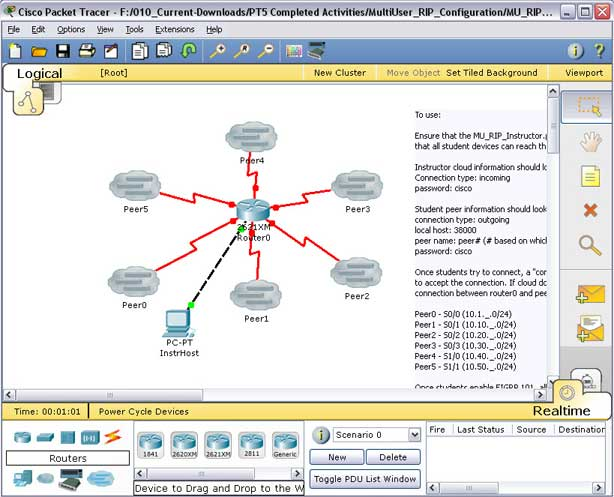
\includegraphics[width=7cm]{figures/r_cpt}
\caption{Cisco Packet Tracer}
\label{fig:r_cpt}
\end{center}
\end{figure}

\section{OMNeT++ simulátor} 
Simulační systém OMNeT++ \cite{reserse:omnet_hp} je velmi propracovaný opensource nástroj pro simulaci prakticky čehokoliv. OMNeT++ je postaven na modulární architektuře, takže při správných knihovnách (modulech) může simulovat počítačovou síť. Systém dokáže simulovat Cisco IOS i počítač postavený na linuxu. Aplikace je komplikovaná a představu jednoduchého programu pro výuku studentů spíše nesplňuje.

Více se tímto simulátorem zabýval Bc. Jan Michek v~rámci své diplomové práce Emulátor počítačové sítě \cite{reserse:omnet_dp}.

\begin{figure}[h]
\begin{center}
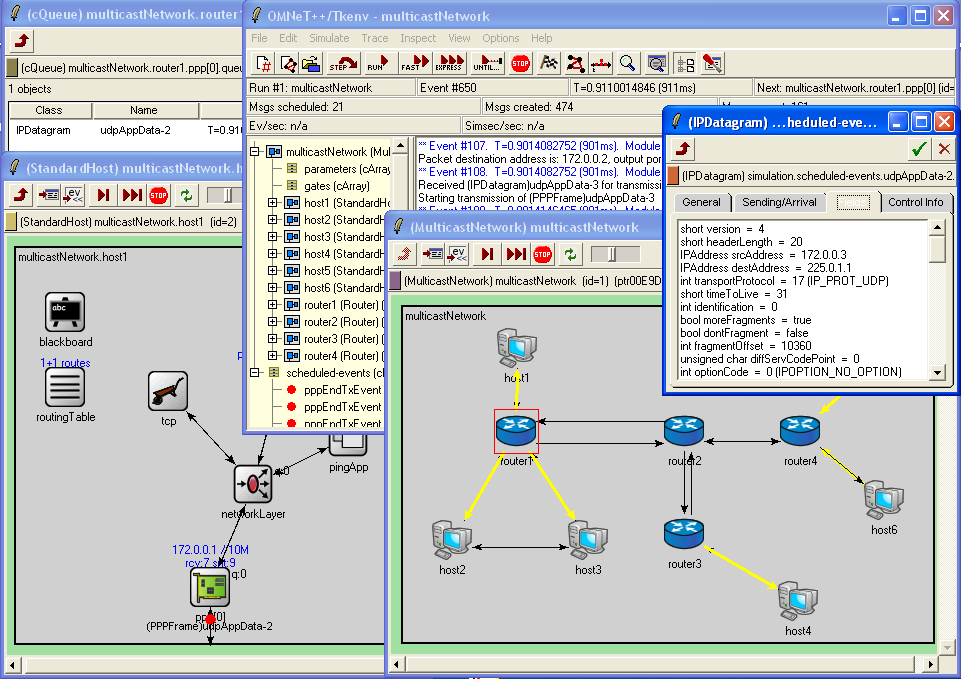
\includegraphics[width=7cm]{figures/r_omnet}
\caption{OMNeT++ simulátor}
\label{fig:r_omnet}
\end{center}
\end{figure}


\section{Simulation Toolkit 7.0} 
Simulation Toolkit 7.0 \cite{reserse:adventnet} je grafický simulátor pro testování a výuku různých síťových aplikací. Simulation Toolkit umožňuje simulaci více než 50000 SNMP služeb (v1, v2c, v3), TL1\footnote{Transaction Language 1}, TFTP\footnote{Trivial File Transfer Protocol }, FTP\footnote{File Transfer Protocol}, Telnet a Cisco IOS na jediném počítači. Software je nabízen pod shareware licencí a je dostupný pro operační systémy Windows, Linux i Unix. Za poskytnutí osobních údajů lze stáhnout plně funkční zkušební verzi na 30 dní. Plná časově neomezená verze stojí od \$995 do \$14995 \footnote{k datu 23.5.2010}.


\section{Boson NetSim Network Simulator} 
Boson NetSim Network Simulator \cite{reserse:boson} je aplikace pro simulaci síťového hardware a software a je designován jako výuková pomůcka pro začínající administrátory Cisco IOS. Systém dokáže simulovat více než 40 různých síťových prvků od firmy Cisco Systems. Simulátor obsahuje grafický i textový konfigurační režim sítí. Program je dostupný pro Windows, Linux i Solaris. Podobně jako Simulation Toolkit i tento software je nabízen ve zkušební verzi na 30 dní. Plná časově neomezená verze stojí od \$99 do \$349 \footnote{k datu 23.5.2010}.

\begin{figure}[h]
\begin{center}
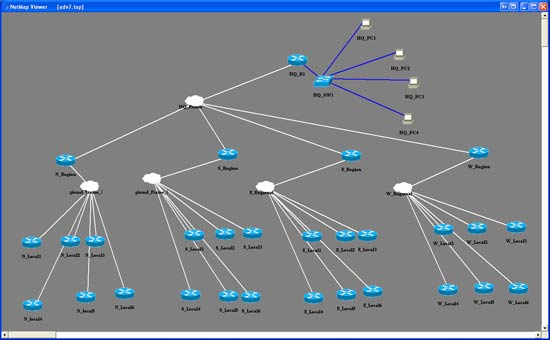
\includegraphics[width=7cm]{figures/r_boson}
\caption{Boson NetSim Network Simulator}
\label{fig:r_boson}
\end{center}
\end{figure}

\section{Dynamips Cisco 7200 Simulator}
Dynamips Cisco 7200 Simulator \cite{reserse:dynamips} je program napsaný Christophe Fillot za účelem emulace Cisco směrovačů. Dynamips funguje na platformách Linux, Mac OS X, Windows a emuluje hardware Cisco směrovačů tak, že se načte obraz originálního Cisco IOS do emulátoru. Program tedy umožňuje využívat veškeré funkce Cisco IOS. Program je licencován pod GNU GPL\footnote{licence pro svobodný software}, ale obraz IOSu není bohužel volně k~dispozici. Tudíž lze program legálně používat jen jako účastník kurzu CNA\footnote{Cisco Networking Academy} - to ale studenti obvykle nejsou, takže tento software také není vhodný pro výuku.

\begin{figure}[h]
\begin{center}
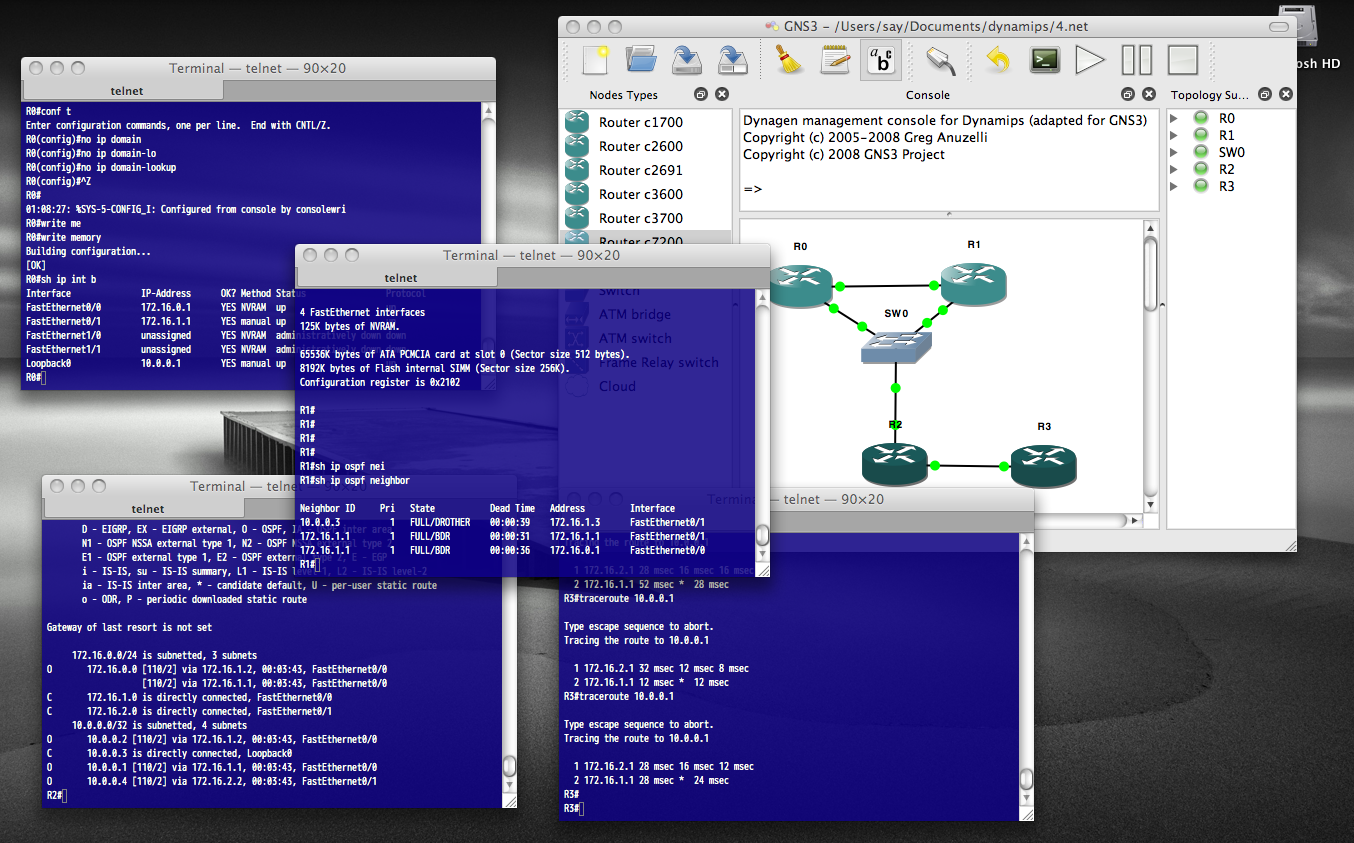
\includegraphics[width=7cm]{figures/r_dynamips}
\caption{Dynamips Cisco 7200 Simulator}
\label{fig:r_dynamips}
\end{center}
\end{figure}

\newpage

\section{Virtuální laboratoř počítačových sítí VirtLab}
Projekt VirtLab \cite{reserse:virtlab} zpřístupňuje laboratorní prvky pro praktickou výuku počítačových sítí vzdáleně prostřednictvím internetu. Studenti ostravské VŠB-TU\footnote{Vysoká škola báňská - Technická univerzita Ostrava} mají možnost si rezervovat pomocí webového rozhraní laboratorní síťové prvky na určitý časový interval a po té k~nim přistupovat přes webový prohlížeč pomocí Java appletů. Propojení síťových prvků se provede automaticky dle zvolené úlohy. Dle mého názoru je to systém velmi ambiciózní, nicméně pro výuku Y36PSI v~praxi nepoužitelný\footnote{Za předpokladu že ČVUT nenaváže spolupráci s~VŠB-TU Ostrava.}.





\chapter{Analýza a~návrh řešení}\label{kap:analyza}
% Analýza a~návrh implementace (včetně diskuse různých alternativ a~volby implementačního prostředí).

% Architektura
%   pocatecni navrh
%   novy navrh: klient - server
%   telnet
%   diskuze nad nacitanim a ukladanim
%   Smerovani + RT (stary navrh - 1 spolecna, novy navrh - wrapper) + prijem paketu
%   NAT 
% Podobnost simulátoru
% Předpokládaný rozsah
% Programovací jazyk
% Paměťová náročnost
% Uživatelské rozhraní


% Jádro aplikace bylo vytvářeno ve spolupráci s kolegou, tudíž následující řádky týkající se architektury systému se mohou v nějaké podobě objevit i v jeho práci. Práce se úmyslně nezabývá striktně mojí vlastní \uv{Cisco částí}, protože tento systém tvoří jeden celek, který je ovlivněn jeho podsystémy. 

% V této kapitole je popsáno především společné jádro. Návrh a implementace Cisco části je v kapitole Realizace \ref{realizace}.

%------------------------------------------------------------------------------

\section{Architektura}

\subsection{Naivní návrh}
Po zadání projektu jsem vytvořil počáteční návrh aplikace a po konzultaci s kolegou (on si udělal také svůj návrh) vznikl tzv. naivní návrh (viz obrázek \ref{fig:navrh}). Tato prvotní varianta počítala s připojením do skutečné sítě, ale byla zavržena zejména kvůli složitosti takového systému a časové náročnosti implementace. Navíc napojení na reálnou síť nepatří mezi požadavky.

\begin{figure}[h]
\begin{center}
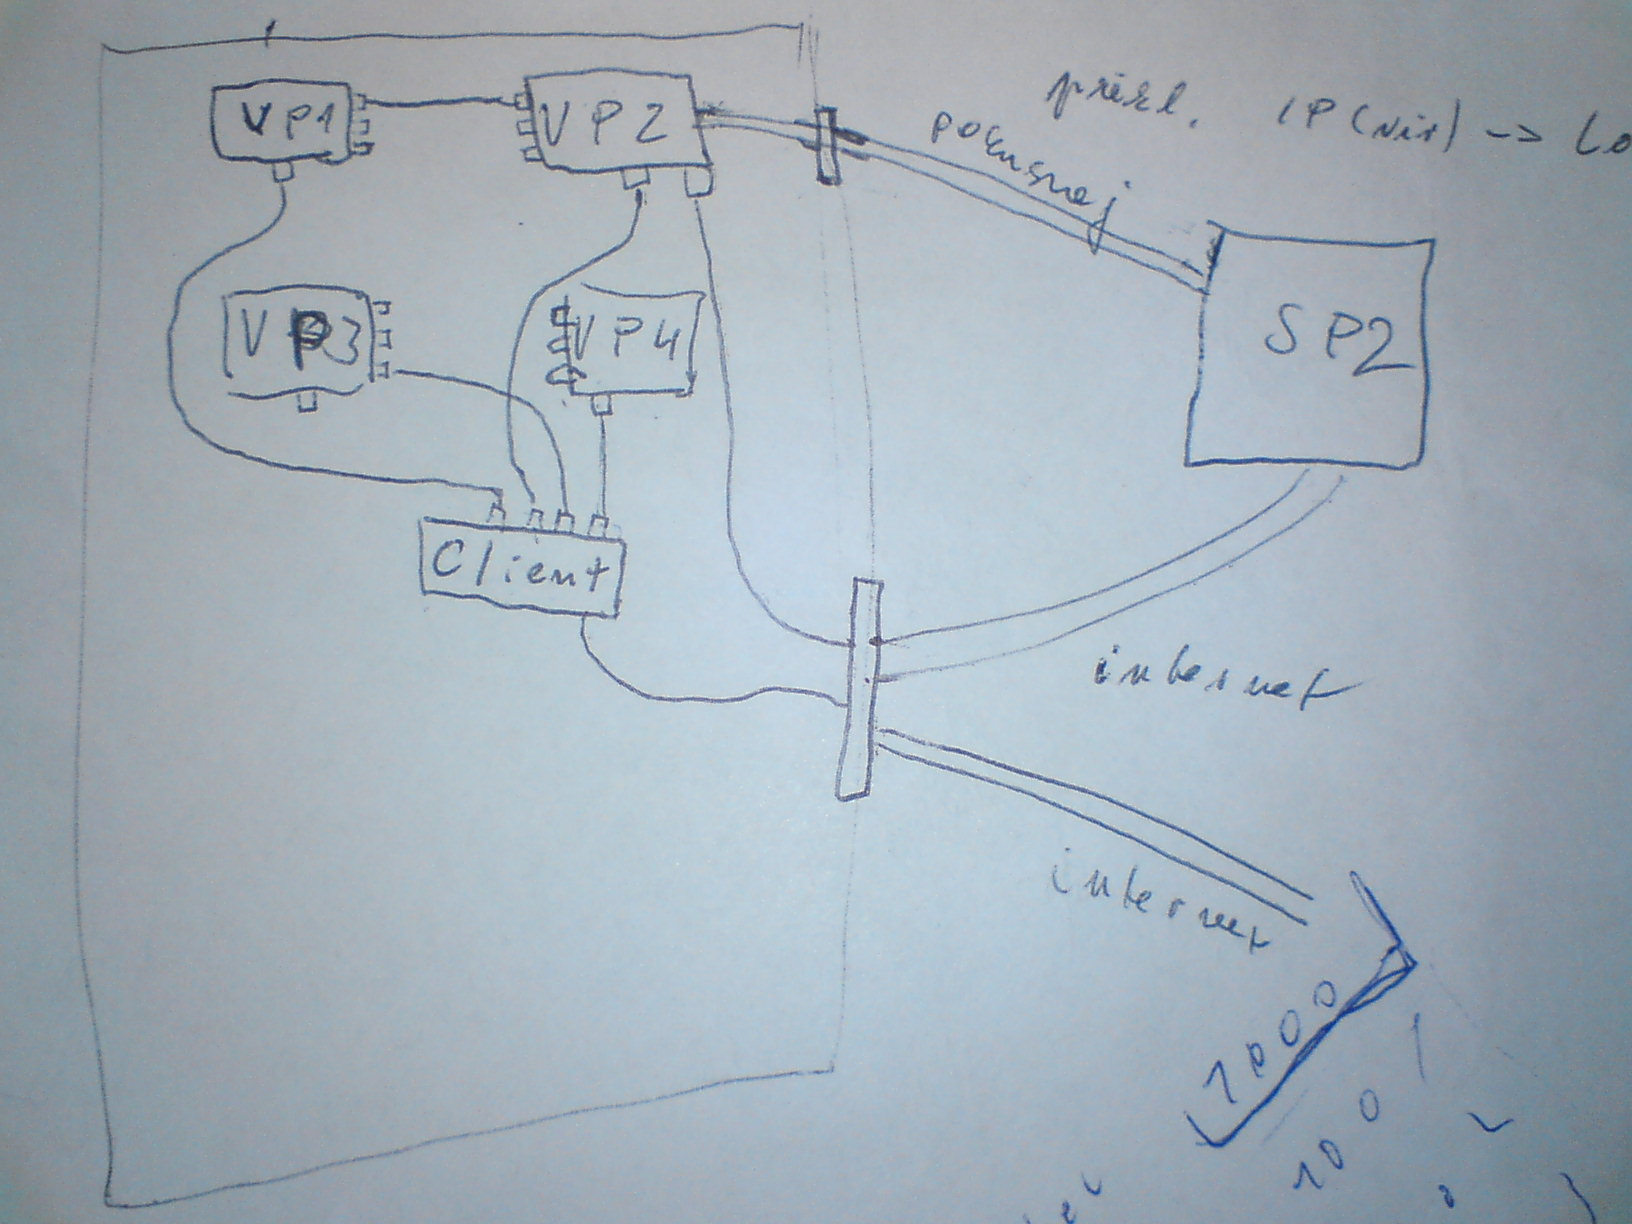
\includegraphics[width=12cm]{figures/navrh}
\caption{Počáteční návrh}
\label{fig:navrh}
\end{center}
\end{figure}

%------------------------------------------------------------------------------

\subsection{Klient - server}\label{klient_server}
Dle nového návrhu bude celá aplikace rozdělena na dvě vrstvy:
\begin{itemize}
 \item komunikační - bude zajišťovat spojení mezi klientskou a serverovou částí aplikace
 \item aplikační - bude tvořit zbytek systému (směrování, překlad adres, parsery příkazů, ..)
\end{itemize}

\subsubsection{Komunikační vrstva}
Komunikační vrstva bude složena z architektury klient - server. Tato vrstva bude převzata ze semestrální práce pro předmět \verb|Y36PSI|, kde bylo za úkol mimo jiné implementovat více-vláknový server. V této převzaté implementaci je server, na kterého se připojují klienti. Pro každého klienta se vytvoří nové vlákno, takže není problém obsluhovat více klientů zároveň. 

Cílem aplikace je vytvořit simulátor počítačové sítě, ta bude muset být zastoupena zřejmě objekty zastupující jednotlivé počítače. A každý počítač se bude muset chovat jako server, aby se na něj mohlo připojit více klientů najednou. Tak bude splněn jeden z funkčních požadavků.

Pro připojení klientů bude použit program \verb|telnet|. Více o návrhu v kapitole \ref{telnet}. 


\subsubsection{Aplikační vrstva}
Tuto vrstvu bude tvořit především parser příkazů emulující Cisco IOS, směrování paketů, routovací tabulka a překlad adres. Aplikační vrstva bude kvůli větší přehlednosti více rozebrána v kapitole Realizace \ref{realizace}.

%------------------------------------------------------------------------------

\subsection{Telnet} \label{telnet}
V zadání je přímo zmíněno použití programu telnet pro připojení klientů k serveru. Telnet je ale také protokol, po kterém se domlouvá telnet klient a telnet server. Česká wikipedie píše o telnet protokolu: \uv{\textit{Protokol přenáší osmibitové znaky oběma směry (duplexní spojení) a je velmi jednoduchý.}\cite{wiki:telnet}}. Podle protokolu se vše posílá po znaku a protistrana po znaku vše potvrzuje. Protokol telnet ale úplně jednoduchý není. Podporuje několik režimů (módů), při navazování spojení začne proces vyjednávání atd. 

Samotný telnet (ať protokol či program) ale neposkytuje doplňování příkazů nebo alespoň historii příkazů. Dalším problémem je, že při psaní příkazů přes telnet nefunguje editace aktuálního řádku, respektive lze mazat po znacích klávesou \verb|BackSpace|, ale nelze se pohybovat do stran šipkami doleva a doprava - při takovém pokusu to vypíše \verb|^[[D| či \verb|^[[C|. 

Napadlo mě zkusit posílat nějaké speciální znaky pro posun kurzoru do stran, aby server věděl, že má nastat posun vlevo či vpravo. Pak by si musel server pamatovat, na které pozici řádku je klient. Nepřišel jsem však na způsob, jak přesvědčit program telnet pro posílání nějakého znaku na událost \uv{šipka doprava}, takže tento návrh jsem musel zavrhnout.

Posun kurzoru se ale neprojevuje při připojování na vlastní telnet server. To je způsobeno tím, že v takovém případě se o editaci řádku a historii příkazů stará samotný server - v mém případě telnet server a BASH\footnote{Bourne again shell - nejpoužívanější unixový shell}. V této aplikaci toho ale nelze využít, takže musí být tyto funkcionality na straně klienta, který je bude zajišťovat. 

Pro Linux jsem našel program rlwrap (readline wrapper), který přidává všechny tyto užitečné funkce: editace řádky, historie příkazů, doplňování příkazů, obarvení promptu. Pro Windows jsem nic takového nenašel, takže uživatelé OS Windows budou muset tuto aplikaci spouštět přes program Cygwin. Výhodou tohoto řešení je lepší uživatelský komfort v příkazové řádce Windows, jelikož program \verb|cmd| je velmi omezen.

%------------------------------------------------------------------------------

\subsection{Konfigurační soubor}
Při startu serveru by se měla načíst konfigurace ze souboru a měla by být možnost uložit aktuální konfiguraci zpět do stejného souboru. Diskuze nad možnými řešeními je popsána v kapitole \ref{xml_soubor}.

%------------------------------------------------------------------------------

\subsection{Směrovač}
Na skutečné počítačové síti jsou síťové prvky několika druhů (switche, bridge, repeatery, směrovače, ..), ale na laboratorních cvičeních předmětu Y36PSI se  nastavují pouze směrovače ze 3. vrstvy\footnote{Tato \uv{síťová vrstva} se stará o směrování v síti a síťové adresování. Dále poskytuje spojení mezi vzdálenými sítěmi, které spolu přímo nesousedí.} síťového ISO/OSI modelu. Proto tato práce bude implementovat pouze jeden typ síťového prvku - směrovač (router). 

%------------------------------------------------------------------------------

\section{Podobnost simulátoru se skutečným směrovačem}\label{kap:podobnost}
Jedním z cílů projektu je vytvořit systém, který bude co nejvíce podobný skutečnému Ciscu. Bude ale potřeba položit někde hranici mezi složitostí a věrností výsledné práce, protože tyto dvě metriky jsou vzájemném protikladu. Cisco IOS je natolik robustní a propracovaný systém, že je v mých silách pouze implementace úzké části systému, která je nutně potřeba pro splnění cíle. Pravděpodobně budu nucen místy ustoupit a nechat vypsat hlášení, že to či ono není v mé implementaci podporováno. 

V samotném parseru příkazů pro Cisco IOS nebude toto téměř vůbec řešeno, protože by to znamenalo implementaci několika stovek pravidel pro všechny příkazy - např. příkaz \verb|ip| má 103 možností v konfiguračním stavu. Aby ale uživatel měl alespoň nějakou možnost se dopátrat, co je podporováno a co ne, tak bude přidán příkaz \verb|help| (\verb|help_en| pro výpis v angličtině), který bude popisovat, co lze v jakém stavu Cisca použít.

%------------------------------------------------------------------------------

\section{Předpokládaný rozsah}
Celý projekt by měl být v rozsahu zhruba 10000 řádků kódu. Nejrozsáhlejší třídy budou pravděpodobně datové struktury pro všechny objekty, které budou emulovat skutečné počítače s rozhraními, routovací a NAT tabulku a mnoho dalších.

%------------------------------------------------------------------------------

\section{Programovací jazyk a prostředí}
Pro implementaci simulátoru jsem si zvolil programovací jazyk Java hned z několika důvodů. Jazyk je to velmi robustní s bohatou sadou různých knihoven. Navíc programy vytvořené v tomto jazyce jsou zpravidla jednoduše přenositelné mezi různými operačními systémy, což je jeden z bodů nefunkčních požadavků. Jazyk Java disponuje propracovaným systémem výjimek, takže při nějaké neočekávané chybě se dozvím víc, než v jazyce C++ s jeho \verb|Segmentation fault|. Neméně významným důvodem je i skutečnost, že s Javou mám zatím největší zkušenosti.

Celá práce bude implementována v Netbeans IDE\footnote{Integrated Development Environment} verze 6.8.

%------------------------------------------------------------------------------

\section{Paměťová náročnost}
Paměťová náročnost bude pravděpodobně vyšší než při použití jazyka C++, jelikož javovský garbage collector není úplně ideální řešení pro uvolňování paměti. Nicméně se neočekává použití tohoto simulátoru pro více než pár desítek virtuálních počítačů, takže spotřeba paměti by neměla překročit požadavky pro běžné aplikace v Javě. Zaplnění paměti touto aplikací by mohlo být kolem 10-30MB (+ načtené prostředí JRE).

%------------------------------------------------------------------------------

\section{Uživatelské rozhraní}
Uživatelské rozhraní by mělo být v zásadě velmi jednoduché. Vše bude ovládáno přes příkazovou řádku, tak jako na skutečném ciscu. Spuštění serveru bude ulehčeno pomocným skriptem \verb|start_server.sh|, který zároveň bude obsahovat nápovědu. Pro připojování klientů budou připraveny rovněž skripty. 

Na obrázku \ref{fig:uziv_rozh} je příklad, jak by mohlo uživatelské rozhraní vypadat pod operačním systémem Linux.

% V balíčku programu Cygwin je rlwrap starší verze, která neumožňuje obarvování promptu a přeposílání signálů (např. při zmáčknutí Ctrl+C nebo Ctrl+Z). Novější verze už tyto funkce mají. Skripty pro připojení na \verb|linux.sh| a \verb|cisco.sh| fungují nezávisle na verzi.

\begin{figure}[h]
\begin{center}
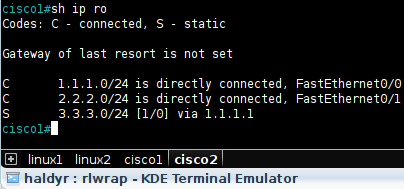
\includegraphics[height=2.5cm]{figures/uziv_rozhrani}
\caption{Uživatelské rozhraní pro konfiguraci cisca}
\label{fig:uziv_rozh}
\end{center}
\end{figure}

%------------------------------------------------------------------------------

% \section{Skutečné Cisco}
% Jedním z největších \uv{oříšků} této práce bylo zjistit, jak se chová skutečné Cisco. Pravdou je, že Cisco Systems má na svých stránkách slušnou řadu návodů, nicméně není tak jednoduché v nich najít, co zrovna potřebujeme. A tak jsem hodně věcí zjišťoval z živého Cisca umístěného na Karlově náměstí přes protokol ssh. 









\chapter{Realizace} \label{realizace}
% Popis implementace/realizace se zaměřením na nestandardní části řešení.
% A tady budu řešit jednotlivé Cisco příkazy - jak jsem na to přicházel, postupné problémy, moje implementace a odchylky.

% \begin{itemize}
%  \item směrování prijmiEthernetove()
%  \item wrapper pro routovací tabulku
%  \item překlad adres
%  \item příkaz Uloz
%  \item SAXHandler
%  \item CiscoParserPrikazu
%  \item Cisco příkazy
%     \begin{itemize}
%      \item Parsery
%      \item ???
%     \end{itemize}
% \end{itemize}

Předkem všech tříd systému na aplikační vrstvě je \verb|Abstraktni|, která zastřešuje převážně statické funkce např. \verb|zaokrouhli| (na tři desetinná místa), \verb|cekej| (metoda pro uspání vlákna, užitečná při výpisech Cisco IOS) a další. Od \verb|Abstraktni| dědí abstraktní \verb|ParserPrikazu|, který seskupuje všechny parsery příkazů (v současné době pro Linux a Cisco IOS). Společný předek Linux a Cisco příkazů je \verb|AbtraktniPrikaz|, z kterého dědí linuxové příkazy kolegy a hlavně \verb|CiscoPrikaz|, který ještě přidává speciálné metody jen pro Cisco příkazy. Viz obrázek \ref{uml:abstraktni}.

\begin{figure}[h]
\begin{center}
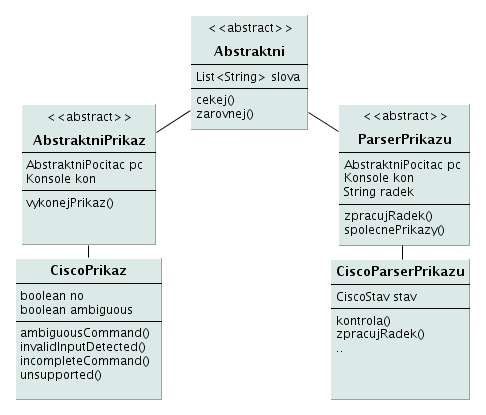
\includegraphics[width=9cm]{figures/uml_abtraktni.png}
\caption{Třídní model předků}
\label{uml:abstraktni}
\end{center}
\end{figure}

Téméř všechny části systému obsahují tzv. debugovací mód, který vypisuje extra informace, co se právě děje nebo přidává další vlastnost vhodnou pro ladění.

\section{Parser Cisco}
Po návrhu a implementaci jádra systému se moje úsilí přesunulo k parseru příkazů pro Cisco. 
% Metoda \verb|zpracujRadek()| je klíčová, protože to je právě ona, kdo rozhoduje, komu bude předáno řízení programu. 

\subsection{Cisco IOS}
Cisco IOS je operační systém, který se nachází na drtivé většině směrovačů firmy Cisco Systems. IOS obsahuje pouze ovládání přes příkazový řádek - CLI\footnote{Command Line Interface}. Pro mě je to spíše výhodou, protože je to mnohem jednodušší na implementaci ve srovnání s \uv{klikacím} GUI\footnote{Graphical User Interface}. IOS má implementováno tzv. zkracování příkazů, které zefektivňuje práci s celým systémem. Celé to funguje tak, že když uživatelův začátek příkazu lze doplnit na jedinečný příkaz (samotné doplnění přes klávesu \verb|TAB|), tak to takový příkaz hned zavolá. Například příkaz \verb|sh run| lze jednoznačně doplnit na \verb|show running-config|, ale kratší \verb|sh ru| už ne:
\begin{verbatim}
Router#sh ru?
rudpv1  running-config
\end{verbatim} 

IOS tvoří několik stavů, např.:
\begin{itemize}
 \item uživatelský mód
 \item privilegovaný mód
 \item konfigurační mód - zde se nastavují volby, které ovlivní celý systém
 \item konfigurace rozhraní - konfigurace jednoho určitého rozhraní
\end{itemize}

\begin{figure}[h]
\begin{center}
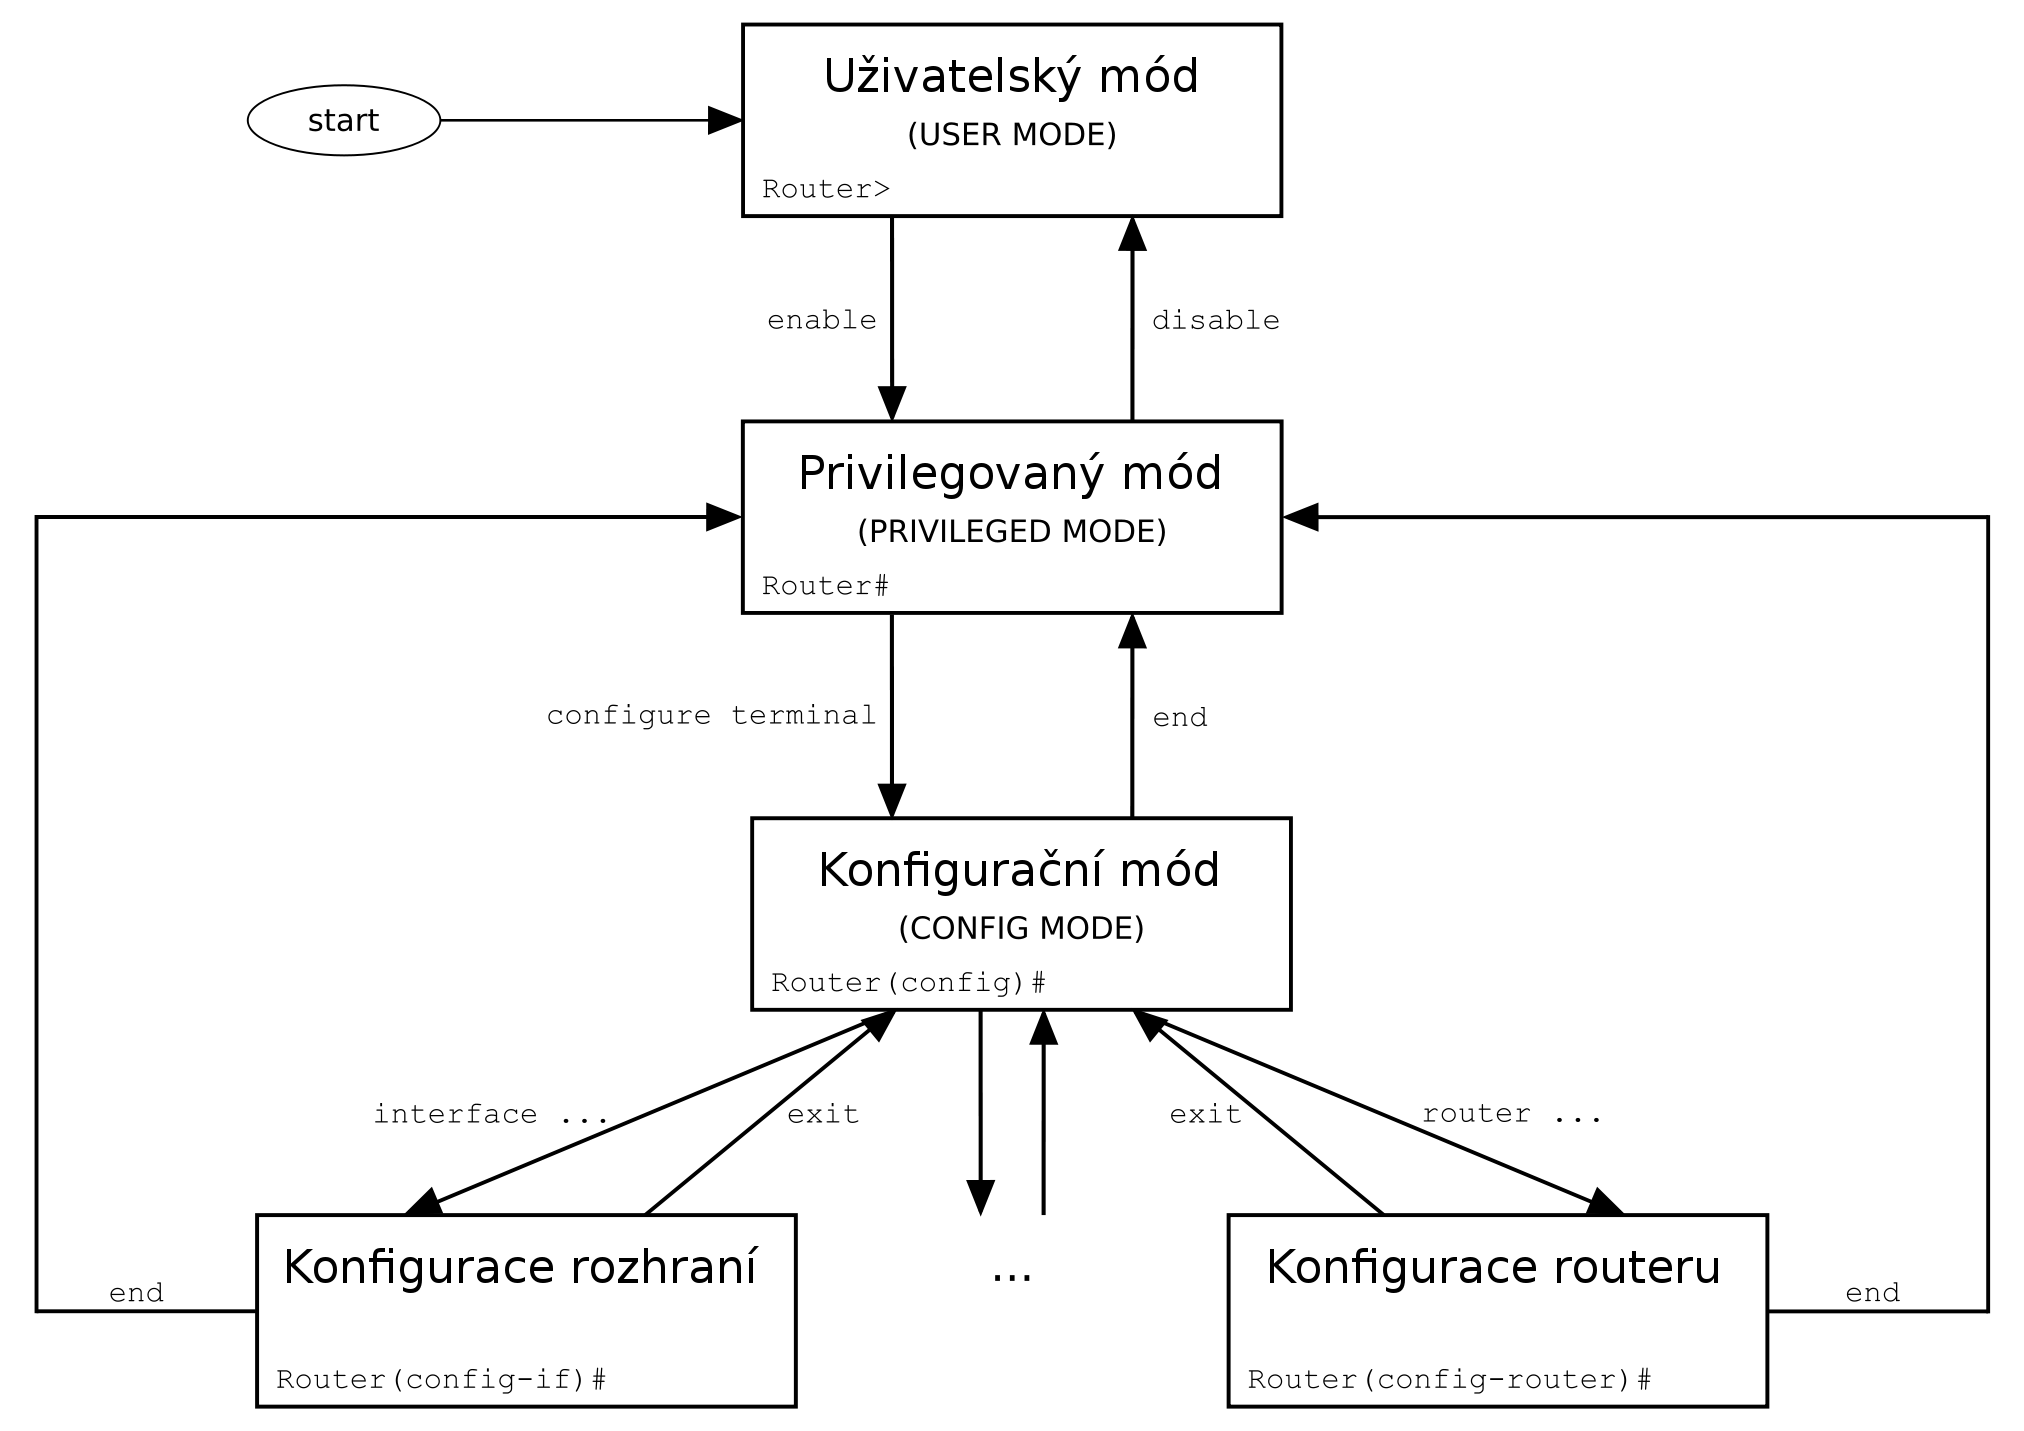
\includegraphics[width=13cm]{figures/ios.png}
\caption{Přehled základních módů Cisco IOS \cite{wiki:ios}}
\label{fig:ios}
\end{center}
\end{figure}

Na obrázku \ref{fig:ios} jsou zobrazeny důležité stavy IOS a přechody mezi nimi. 

\subsubsection{Uživatelský mód}
Uživatelský mód (USER MODE) je výchozí (startovací) mód. Tento mód je značně limitovaný a dovoluje použití čistě read-only příkazů (tj. takových, které nezmění konfiguraci). Přesto má tento mód svoje opodstatnění, dovoluje např. výpis směrovací tabulky \verb|show ip route| či příkazy \verb|ping| nebo \verb|traceroute|. Do privilegovaného režimu se lze přepnout příkazem \verb|enable|.

\subsubsection{Privilegovaný mód}
Privilegovaný mód (PRIVILEGED MODE) nebo také \uv{administrátorský} mód je podobný linuxovému \verb|root| účtu. Tento mód je výchozím bodem pro vstup do ostatních módů. Pro návrat zpět do uživatelského režimu existuje příkaz \verb|disable|. Příkaz \verb|configure| způsobí přepnutí do dalšího konfiguračního módu. Tento stav umožnuje vypsat veškeré informace o aktuální konfiguraci systému, např.:
\begin{itemize}
 \item \verb|show running-config| - shrnutí aktuální konfigurace
 \item \verb|show ip route| - výpis směrovací tabulky
 \item \verb|show ip nat translations| - výpis dynamických záznamů v NAT tabulce
\end{itemize}
Není důvod, proč by v tomto stavu nefungovaly příkazy \verb|ping| a \verb|traceroute|.

\subsubsection{Konfigurační mód}
Konfigurační mód (CONFIG MODE) je jeden z nejdůležitějších, protože umožňuje konfiguraci směrovacích záznamů (\verb|ip route|), přístupových seznamů pro potřeby překladu adres (\verb|access-list|), pooly IP adres (\verb|ip nat pool|) a výběr rozhraní pro přechod do stavu konfigurace rozhraní (\verb|interface|).

\subsubsection{Konfigurace rozhraní} \label{configif}
V tomto módu lze nastavovat IP adresy na aktuálně vybrané rozhraní, nastavovat příznaky pro veřejné a soukromé rozhraní pro NAT (\verb|nat inside|, \verb|nat outside|) nebo také zapínat či vypínat rozhraní. Pro přechod ze všech konfiguračních módů do privilegovaného stačí napsat příkaz \verb|end| nebo jen stisknout klávesovou zkratku \verb|Ctrl+Z|.


\subsection{Implementace Cisco IOS}
Cisco IOS obsahuje desítky příkazů z nichž každý může mít až stovky variací. Proto jsem implementoval pouze úzkou část příkazů, která je potřebná pro splnění zadání této práce. Nejdůležitější funkcí parseru je rozpoznávání zkrácených příkazů. Na skutečném Ciscu se opravdu procházejí všechny možnosti, které mohou v daném stavu nastat, a podle nich probíhá vyhodnocování. V mé implementaci ale mám pouze část příkazů, takže jsem to musel vyřešit jiným způsobem. Pro každé slovo (část příkazu) si \verb|CiscoParserPrikazu| drží počet písmen, který je potřeba k jednoznačnému určení příkazu. Tato čísla jsem \uv{naměřil} na školních ciscách v březnu 2010. Zajímavé je, že už o 2 měsíce později jsem objevil drobné změny. Čísla se mohou měnit s různými verzemi Cisco IOS. To bych ale neviděl jako zásádní problém. Většina studentů (alespoň dle mé zkušenosti) stejně píše celé příkazy a zkrácené verze nepoužívá.

Vyhodnocování příkazů zajišťuje metoda \verb|kontrola(command, cmd)|. Parametr \verb|command| je celý příkaz, na který by se to mohlo eventuelně doplnit, a \verb|cmd| je příkaz poslaný od uživatele. Nejdříve se zjistí počet znaků, který je potřeba pro jednoznačné doplnění na příkaz \verb|command|. Po té se zkontroluje požadovaný počet znaků a také jestli zkrácený příkaz odpovídá doplněnému. A jak to vypadá v kódu:

\begin{verbatim}
if (cmd.length() >= i && command.startsWith(cmd)) {
    // lze doplnit na jeden jedinecny prikaz
    return true;
}
if (command.startsWith(cmd)) {
    // vypsat amiguous command
    nepokracovat = true;
}
\end{verbatim}

Jednotlivé příkazy Cisco IOS jsou implementovány v samostatných třídách. Třída \\\verb|CiscoParserPrikazu| tedy zajišťuje přechody mezi stavy (módy) a \uv{nahazování} rozhraní. Přepnutí stavu rozhraní je natolik triviální, že se by se nevyplatilo mít pro to zvláštní třídu. 

\paragraph{}
Ladící mód zjednodušuje testování parseru a přidává tyto funkce:
\begin{itemize}
 \item klávesa \verb|Enter| funguje jako přechod z uživatelského do privilegovaného módu
 \item použití příkazů z jiných módů v privilegovaném módu - navíc např. \verb| ip route|, \\\verb|ip nat pool inside|, \verb|access-list|, ..
 \item extra výpis dynamických záznamů v natovací tabulce
 \item výpis \verb|show running-config| je pro přehlednost zkrácen
 \item možnost testování routovací tabulky přes linuxový příkaz \verb|route|
 \item používání linuxového příkazu \verb|ifconfig|
\end{itemize}
Použití těchto věcí je vhodné spíše pro ladění programu do budoucna než pro běh v \uv{ostrém} provozu. Tento mód je ve výchozím stavu vypnut.

\subsection{Odchylky v implementaci}
Má implementace Cisco IOS má navíc pár příkazů, které jsou potřeba pro ovládání systému. Jak už jsem se zmiňoval v kapitole \ref{kap:podobnost} je zde navíc \verb|help| a \verb|help_en| pro výpis nápovědy. Příkaz \verb|kill| přijde vhod, když uživatel chce ihned vypnout aplikaci a nechce projít přes několik stavů příkazem \verb|exit|. Další servisní příkaz je \verb|save| nebo také \verb|uloz|, který zapíše aktuální konfiguraci všech počítačů do konfiguračního souboru, se kterým byl spuštěn nebo který byl předán jako parametr. Dále lze využít velmi jednoduchý příkaz \verb|?| (otazník), který vypíše seznam dostupných příkazů v aktuálním stavu.

Na skutečném Ciscu funguje kombinace kláves \verb|Ctrl+Z| pro přechod do privilegovaného módu. Ale kvůli použití programu\verb|rlwrap| je systém limitován. Omezení spočívá v tom, že \verb|rlwrap| přepošle signál operačnímu systému a ten pozastaví tento proces. Proces lze obnovit příkazem fg (na OS Linux), bohužel klientský program \verb|telnet| neumí po pozastavení obnovit svoji funkčnost a přestává posílat vstup na standartní výstup. Je tedy už nepoužitelný a pro tyto přídady existuje příkaz \verb|kill|, který ukončí tento rozbitý proces a klient se může přípojit znova. Lépe je na tom zkratka \verb|Ctrl+C|, která pouze ukončuje (signál SIG\_INT) daný proces a tedy funguje bez problému. 

Program \verb|rlwrap| je ale šířen jako balíček pod programem \verb|cygwin| v zastaralé verzi\footnote{stav z 18.5.2010}, která neumožňuje přeposílání signálů, takže při stisku \verb|Ctrl+C| i \verb|Ctrl+Z| přestane \verb|telnet| klient vypisovat na standartní výstup a nezbývá než použít \verb|kill|.








% \lstinline{System.out.println("Tady je text")}




\section{Načítání ze souboru}
\subsection{Zpracování parametrů}
Po spuštění startovacího skriptu \verb|start_server.sh| se nejdříve zpracují všechny parametry. Když je nalezen parametr \verb|-n|, tak se načítá z konfiguračního souboru pouze kostra sítě s počítačema a rozhraníma bez jejich nastavení. Pozice tohoto parametru není důležitá, systém nejprve detekuje přítomnost tohoto parametr a pak už ho vůbec neřeší. Další parametr je název konfiguračního souboru, ten může být zadán bez koncovky \verb|.xml|, nejdříve se zkusí načíst soubor bez koncovky a když takový soubor není, tak se načte soubor s koncovkou. Třetím parametrem je port, od kterého budou poslouchat jednotlivé počítače. Port je nepovinný, výchozí volba je port 4000. Když je daný port obsazený, tak se program ukončí z chybovou hláškou.

%------------------------------------------------------------------------------

\subsection{Konfigurační soubor}
Nejdříve bylo nutno rozhodnout podobu výsledného konfiguračního souboru. Existuje několik možností, např.:
\begin{itemize}
 \item javovské \verb|Properties| ve stylu \uv{proměnná = hodnota}, moc se nehodí na velmi členité struktury
\begin{verbatim}
compile.on.save=false
do.depend=false
do.jar=true
javac.debug=true
\end{verbatim} 

 \item podoba konfiguračních souborů KDE\footnote{K Desktop Environment je desktopové prostředí pro Linux a další unixové operační systémy.}, kde jednotlivé sekce jsou odděleny jménem v hranatých závorkách
\begin{verbatim}
[Xdmcp]
Enable=false
[Shutdown]
# Default is "/sbin/halt"
HaltCmd=/sbin/shutdown
\end{verbatim} 

 \item XML\footnote{Extensible Markup Language je rozšiřitelný značkovací jazyk} soubor, který umožňuje libovolnou strukturu
\end{itemize}

Já jsem si vybral technologii XML pro jeho robustnost a velmi dobrou čitelnost.

Načítání z XML souboru lze udělat minimálně dvěma způsoby: Vzít cizí knihovnu, která tuto funkcionalitu zajišťuje, nebo vytvořit vlastní třídu. Obě možnosti mají své výhody i nevýhody. Cizí knihovna by mohla být téměř bez práce a pravděpodobně by podporovala i zpětné ukládání. Na druhou stranu by byla malá možnost ovlivnění výsledného výstupu a bylo by vše na té knihovně závislé. Navíc s novými verzemi by se mohla měnit i její funkčnost. Znamenalo by to také instalaci této knihovny na uživatelských počítačích. Z těchto důvodů jsem zvolil druhou variantu: vlastní implementace zpracování XML. 

%------------------------------------------------------------------------------

\subsection{Implementace SAX handleru}
Zpracovat XML lze přes technologii DOM\footnote{Document Object Model} a SAX\footnote{Simple API for XML}. Já se rozhodl pro SAX z těchto důvodů:
\begin{itemize}
 \item jednorázové sekvenční čtení - vyšší rychlost
 \item menší paměťová náročnost
 \item oproti DOMu i několikrát rychlejší, což u velmi rozlehlé síťě by mohlo být znatelné
\end{itemize}

Můj \verb|SAXHandler| tvoří tři části: samotné načítání, datová struktura pro počítač a vytváření virtuálního počítače.

\subsubsection{Načítání}
\verb|ContentHandler| vyhazuje události při zpracování XML souboru. \verb|SAXHandler| musí tyto události odchytávat a pokud je to událost, která nás zajímá, tak se zpracuje tj. uloží do datové sktruktury. Musí být implementovány metody na zpracování začátku elementu, konce elementu, znaková data a konce dokumentu. Po načtení konce elementu se vytvoří virtuální síť počítačů. Pro správnou funkci \verb|SAXHandler| je důležité mít ve složce s konfiguračními soubory také soubor DTD\footnote{Document Type Definition}, který definuje strukturu XML dokumentu.

\subsubsection{Datová struktura}
Pro ukládání informací slouží datová struktura \verb|PocitacBuilder|, která si drží veškeré informace načtené z XML souboru o jednom počítači:
\begin{itemize}
 \item jméno a typ počítače
 \item nastavení rozhraní - jméno, adresa, maska, stav
 \item routovací tabulka - výčet záznamů
 \item ip\_forward - pro potřeby Linuxu
 \item překlad adres - pooly adres, access-listy, přiřazení access-listů k poolům, statické záznamy
\end{itemize}

Pak je tu ještě sekundární struktura pro uložení kabelů k jednotlivým počítačům.

\subsubsection{Vytváření virtuálních počítačů}
Po vyhození události konec souboru se začnou vyrábět virtuální počítače. Pokud byl použit parametr \verb|-n|, tak se nejdříve smažou nastavení, která nemají být načtena. Po té se postupně budou načítat (a kontrolovat) všechny uložené nastavení. V zásadě lze říci, že když systém narazí na neplatná data v konfiguračním souboru, tak vypíše chybovou hlášku na standardní chybový výstup. Pokud je to chyba zásadní, tak se vyhodí výjimka, vypíše hláška a celý server se ukončí, protože nemůže pokračovat v další činnosti. Slovem zásadní je myšleno např. chybějící jméno rozhraní (kabely v XML jsou napojeny přes jména rozhraní), natažená kabeláž a opakující se jména počítačů či rozhraní na jednom počítači. Kabely jsou natolik klíčovou věcí, že uživatele upozorní na chybu pádem programu s výpisem, co je špatně. 

Takto vypadá příklad konfiguračního souboru:
\begin{verbatim}
<pocitac jmeno="cisco1" typ="cisco">
  <rozhrani>
    <jmeno>FastEthernet0/0</jmeno>
    <ip>192.168.1.254</ip>
    <maska>255.255.255.0</maska>
    <mac>00:0b:0c:0d:0a:01</mac>
    <nahozene>true</nahozene>
    <nat>soukrome</nat>
  </rozhrani>
...
\end{verbatim} 

%------------------------------------------------------------------------------

\section{Ukládání do souboru}
Abstraktní \verb|ParserPrikazu| obsahuje metodu, do které jsou vloženy všechny společné příkazy. V současné době je tam pouze příkaz \verb|uloz| alias \verb|save|. Uživatel může použít jakoukoliv variantu dle libosti. Při zavolání tohoto příkazu bez parametru se bude ukládat do stejného souboru, ze kterého se při staru aplikace načítalo. Nebo může uživatel specifikovat jméno souboru (včetně cesty), do kterého se má aktuální konfigurace uložit. 

Ukládání do souboru je realizováno čistě textově, tzn. vše se posílá přes \verb|BufferedWriter| bez použítí externích knihoven. Pro usnadnění práce jsem si napsal několik pomocných metod, kde např. pro uložení MAC adresy do XML stačí zavolat \\\verb|zapisElement("mac", rozhrani.macAdresa)|. Velmi užitečná metoda je také \verb|vratElement|, která postaví element s daným jménem a obsahem:
\begin{verbatim}
private String vratElement(String jmeno, String obsah) {
  if (obsah == null) {
    obsah = "";
  }
  return "<" + jmeno + ">" + obsah + "</" + jmeno + ">\n";
}
\end{verbatim} 


Výhodou tohoto řešení je maximální kontrola nad výstupem příkazu a jednudochost implementace. Mezi nevýhody bych uvedl hlavně změnu v datových strukturách. Když by bylo potřeba připsat novou volbu, která by se měla ukládat do XML souboru, tak musíme přidat pravidla pro načítání z XML v \verb|SAXHandler| a navíc zde ukládání.



\section{Směrování} \label{prijmiEthernetove}
Směrování implementoval kolega, nicméně se Cisco nechová vždy stejně, a tak bylo nutné vyčlenit rozhodování o příjmu paketů do koncových počítačů a implementovat je každý zvlášť. Nejsložitější bylo zjistit, jak se Cisco přesně chová a proč to tak je. Všechny vyzkoumané informace byly platné v období březen - duben 2010. Někdo předělával školní cisca po tom, co jsem prováděl experimenty, takže je možné, že některé věci se už chovají jinak.

Při různých experimentech jsem zjistil, že když linuxu přijde paket, na který nemá záznam (routu) ve směrovací tabulce, tak pošle zpátky patek \verb|Destination Network Unreachable|, zatímco školní cisca posílají \verb|Destination Host Unreachable|.

Při testování standardních případů je vše jasné, ale když jsem zkusil síť nakonfigurovat trochu neobvykle, tak to tak jasné nebylo.

%------------------------------------------------------------------------------

\subsection{Debuging}
Na stránkách firmy Cisco Systems jsem objevil několik návodů týkajících se vypisování zpracování paketů na jednotlivých strojích. Bez těchto návodů lze jen těžko hádat, které pakety se posílají kam. Velmi užitečné jsou tyto příkazy:

\begin{itemize}
 \item \verb|debug ip packet detail| - detailní výpis zpracování IP paketů 
 \item \verb|debug ip icmp| - zpracování ICMP\footnote{Internet Control Message Protocol je jeden z nejdůležitějších protokolů ze sady protokolů internetu. Používají ho operační systémy počítačů v síti pro odesílání chybových zpráv, například pro oznámení, že požadovaná služba není dostupná nebo že potřebný počítač nebo router není dosažitelný. \cite{wiki:icmp}} paketů
 \item \verb|debug arp| - výpis ARP protokolu o zjišťování MAC adres sousedních počítačů
\end{itemize}

%------------------------------------------------------------------------------

\subsection{Síť č.1}
\subsubsection{Popis problému}
Vezměme si následující síť \ref{fig:sit_2pc} složenou pouze ze dvou počítačů cisco a linux. Tyto počítače mají nastavené IP adresy z jiných sítí, linux má nastavenou defaultní routu na rozhraní \verb|eth0| a cisco má samo-nastavující se routu na síť, která je přiřazena na rozhraní \verb|F0/0|\footnote{Na obrázcích sítí se vyskytují zkratky F0/0 a F0/1, které značí FastEhernet0/0 resp. FastEhernet0/1}. Samo-nastavující znamená, že cisco přidává záznamy do routovací tabulky podle informací z jeho rozhraní. Tuto funkcionalitu lze vypnout, na školních ciscách je ale defaultně zapnutá. Cisco nenahazuje tuto routu v případě, že na druhém konci kabelu buď nikdo není nebo je shozené (vypnuté) rozhraní.

\begin{figure}[h]
\begin{center}
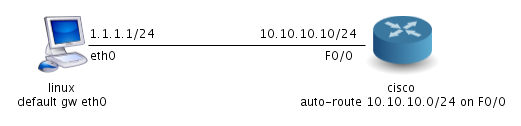
\includegraphics[width=13cm]{figures/sit_2pc.png}
\caption{Síť linux - cisco}
\label{fig:sit_2pc}
\end{center}
\end{figure}

Při připojení na linux a spuštění příkazu \verb|ping 10.10.10.10| se stane, že u prvních pár paketů (při mém testování to bylo 9) vyprší timeout a pak už linux sám sobě vypisuje \verb|Destination Host Unreachable|. Dlouho jsem se snažil přijít na to, proč to tak je. Těžko jsem zjišťoval, co se děje, protože jsem neměl žádné zkušenosti se sledováním paketů přes cisco směrovače. 

\subsubsection{Řešení} 
Nejdříve vysvětlím proč prvních několik paketů prošlo až na cisco a na další \verb|icmp_req| odpověděl linux sám sobě. Je to způsobeno tím, že při prvních paketech ještě cisco nevědělo co s těmi pakety bude, a tak je přijalo, aby mohlo vyhodnotit co dál. Cisco ale hned přišlo na to, že nemá žádnou routu na \verb|1.1.1.1|, takže neví, co s takovými pakety dělat, tak se radši rozhodlo, že je ani nepřijme. Obvykle cisco nepřijímá pakety ihned, ale školní cisca měly starší verzi software a celkově byly zpomalený, takže to bylo způsobeno asi tím.

Linux nejprve pošle ARP request, aby zjistil MAC adresu cisca. Cisco přijme ARP a snaží se odpovědět na dotaz. Problém je, že nemá záznam v routovací tabulce na adresu \verb|1.1.1.1|, takže ani neodpoví na ARP request, tak je \uv{hezky} je nastavené cisco.

%------------------------------------------------------------------------------

\subsection{Síť č.2}
\subsubsection{Popis sítě}
Na další síti \ref{fig:sit_3pc} jsou počítače linux1, cisco1 a cisco2 zapojené do jedné \uv{nudle}. Konfigurace rozhraní a směrovacích tabulek je obsažena v obrázku. Linux1 má teoreticky v dosahu (přes defaultní routu) cisco2, to mu ale nemůže odpovědět, protože pro linux1 nemá záznam. Cisco1 přeposílá pakety z cílovou adresu \verb|8.8.8.0/24| na bránu - cisco2.

\begin{figure}[h]
\begin{center}
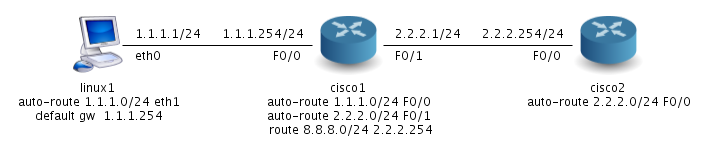
\includegraphics[width=15cm]{figures/sit_3pc.png}
\caption{Síť linux1 - cisco1 - cisco2}
\label{fig:sit_3pc}
\end{center}
\end{figure}

%------------------------------------------------------------------------------

\newpage

\subsubsection{Experimenty} 

\textbf{I. experiment}\\
První experiment je \verb|ping| z linux1 na cisco2:
\begin{verbatim}
linux1:/home/dsn# ping -c2 8.8.8.8
PING 8.8.8.8 (8.8.8.8) 56(84) bytes of data.
From 2.2.2.254 icmp_seq=1 Destination Host Unreachable
From 2.2.2.254 icmp_seq=2 Destination Host Unreachable
\end{verbatim}
Vše dopadlo dle očekávání tedy paket proplul až na vzdálené cisco2, které nemělo pravidlo pro manipulaci paketů s cílem \verb|8.8.8.8|, a tak poslalo zpátky odesílateli \\ \verb|Destination Host Unreachable|.
\newline

\textbf{II. experiment}\\
Pokud zkusíme odeslat \verb|ping| na \verb|1.1.1.2|, což je adresa v síti mezi linux1 a cisco1, ale není to adresa ani jednoho z nás, tak dopadne takto:
\begin{verbatim}
linux1:/home/dsn# ping -c2 1.1.1.2
PING 1.1.1.2 (1.1.1.2) 56(84) bytes of data.
From 1.1.1.1 icmp_seq=1 Destination Host Unreachable
From 1.1.1.1 icmp_seq=2 Destination Host Unreachable
\end{verbatim} 
Linux ví (díky ARP protokolu), že vedle něj není počítač s IP adresou \verb|1.1.1.2|, a tak se to ani nesnaží odeslat. Je to zapříčiněno také tím, že routa \verb|1.1.1.0/24| je na rozhraní a ne na gateway.
\newline

\textbf{III. experiment}\\
Cisco má trochu odlišné chování:
\begin{verbatim}
cisco1#ping 1.1.1.2

Type escape sequence to abort.
Sending 5, 100-byte ICMP Echos to 1.1.1.2, timeout is 2 seconds:
.....
Success rate is 0 percent (0/5)
\end{verbatim}
Cisco se zeptalo ethernetově (přes ARP) linuxu, ten odpověděl, že takovou adresu nemá a cisco vypsalo \uv{.}, což znamená, že vypršel timeout. Linux poslal \verb|DHU|\footnote{Destination Host Unreachable} a ciscu vypršel timeout.

%------------------------------------------------------------------------------

\newpage

\subsection{ARP protokol} \label{arp}
\uv{Address Resolution Protocol (ARP) se v počítačových sítích s IP protokolem používá k získání ethernetové MAC adresy sousedního stroje z jeho IP adresy. Používá se v situaci, kdy je třeba odeslat IP datagram na adresu ležící ve stejné podsíti jako odesilatel. Data se tedy mají poslat přímo adresátovi, u něhož však odesilatel zná pouze IP adresu. Pro odeslání prostřednictvím např. Ethernetu ale potřebuje znát cílovou ethernetovou adresu.}\cite{wiki:arp}

Z různých experimentů jsem sestavil tato ARP pravidla, podle kterých cisco vyhodnocuje ARP requesty:
\begin{enumerate}
 \item zdrojová IP adresa není ve stejné síti viz obrázek \ref{fig:sit_2pc}, tak se diskartuje ARP request - lze obejít v konfiguraci, tak jsou také nastavená školní cisca
 \item cílová IP adresa nesedí s žádnou s žádnou mojí IP adresou, diskartuje se ARP reply
 \item IP zdroje (tazatele) je dostupná před pravidla v routovací tabulce, tak se vygeneruje ARP reply a pošle se tazateli
\end{enumerate}

%------------------------------------------------------------------------------

\subsection{Pravidla o příjmu paketů} 
Z předchozí sekce \ref{arp} jsem vyvodil několik pravidel pro příjem paketů u počítače cisco. Tato pravidla tvoří de facto tělo metody \verb|prijmiEthernetove| u \verb|CiscoPocitac|.

\begin{itemize}
 \item když mohu odpovědět na ARP request a zároveň je paket pro mě nebo vím kam ho poslat dál, tak se paket přijme
 \item když nelze odpovědět na ARP request = nemám na něj routu ve směrovací tabulce, tak se paket nepřijme
 \item ve všech ostatních případech se paket nepřijme
\end{itemize}




\section{Wrapper směrovací tabulky}
Routovací tabulka, kterou implementoval kolega, je \uv{šitá} pro linux. Abych ji mohl použít, musel jsem vytvořit \verb|CiscoWrapper|, který bude linuxovou tabulku ovládat. Hlavní důvodem pro vytvoření nějakého wrapperu je skutečnost, že cisco svoji routovací tabulku vypočítává z~nahozených rozhraní a ze statických pravidel vložených uživatelem. Má tedy zvlášť datovou strukturu pro statická pravidla a pro samotnou routovací tabulku.

Mohl jsem si implementovat kompletně vlastní routovací tabulku, ale nějaké podobě wrapperu bych se stejně nevyhnul. Byla by to tedy zbytečná práce, která by navíc znamenala určité zdvojení kódu.

%------------------------------------------------------------------------------

\subsection{Směrovací tabulka}
Linuxová routovací tabulka je složena ze záznamů, kde každý z~nich je tvořen těmito položkami: adresát, brána a rozhraní. Existují (pro tuto práci důležité) dva typy záznamů:
\begin{itemize}
 \item záznam na bránu - příznak UG, při přidávání UG záznamu platí, že nově přidávaná brána musí být dosažitelná příznakem U~(= nějakým záznamem na rozhraní)
 \item záznam na rozhraní - příznak U, převážně záznamy od nahozených rozhraní
\end{itemize}

%------------------------------------------------------------------------------

\subsubsection{Výběr záznamů}
Pravidla jsou ukládána do routovací tabulky podle masky - ta je hlavním kritériem. Když je tedy potřeba rozhodnout, který záznam vybrat pro příchozí paket, tak se začne procházet tabulka a vratí se první záznam, kde se shoduje adresát záznamu s~adresátem paketu. Tím zajistíme požadavek cisca, aby se směrovalo vždy podle adresáta s~nejvyšším počtem jedniček v~masce.

\subsection{Wrapper}
\verb|CiscoWrapper| v~podstatě kopíruje datové struktury linuxové routovací tabulky a přidává několik obslužných metod. Největším oříškem byla správná aktualizace routovací tabulky na základě wrapperu. Wrapper si pamatuje statické směrovací záznamy a dle nahozených rozhraní generuje správné záznamy do routovací tabulky. 

\subsubsection{Statické záznamy}
Statické směrovací záznamy se zadávají v~privilegovaném módu přes příkaz \\\verb|ip route <adresa> <maska> <brána OR rozhraní>|. Záznam se nepřidá pouze v~případě neexistujícího rozhraní a adresy ze zakázaného rozsahu. Do zakázaného rozsahu patří IP adresy ze třídy D a E. Třídy adres jsou popsány v~následujícím odstavci. V~dohledné době se začnou uvolňovat IP adresy ze třídy E kvůli nedostatku IPv4 adres. Až se tak stane, tak Cisco bude muset vydat aktualizaci svého IOSu, protože v~něm momentálně nelze přiřazovat adresy z~tohoto rozsahu.
\begin{verbatim}
Třída  Začátek 1. bajt  Maska           Sítí        Stanic v~každé síti
A~0       0–127    255.0.0.0       126         16 777 214
B      10      128-191  255.255.0.0     16384       65534
C      110     192-223  255.255.255.0   2 097 152   254
D      1110    224-239  multicast
E      1111    240-255  vyhrazeno jako rezerva
\end{verbatim}
Upravený výpis s~Wikipedie \cite{wiki:ip} a ověřený z~webu organizace IANA \cite{iana}.

\paragraph{}
Když se přidává záznam s~nedosažitelnou bránou, tak IOS nevypíše žádnou chybovou hlášku (narozdíl od linux, který vypíše \verb|SIOCADDRT: No such process|). Záznam se uloží do wrapperu a je přidán do routovací tabulky ve chvíli, kdy bude dosažitelný. 

Při jakékoliv změně IP adresy na rozhraní či změně statických záznamů se smaže celá routovací tabulka a spustí se aktualizační funkce \verb|update|. Ta nejdříve přidá záznamy na rozhraní (dle nastavených adres vsech rozhraních\footnote{V kapitole \ref{prijmiEthernetove} jsem takovému chování říkal \uv{samo-nastavující záznamy.}}) a pak začne postupně propočítávat jednotlivé záznamy z~wrapperu. Záznam na rozhraní je přidán automaticky pokud výstupní rozhraní není shozené. Záznam na bránu se hledá přes rekurzivní metodu \\\verb|najdiRozhraniProBranu|.

V~mé implementaci je zabudována ochrana proti smyčkám u~záznamů na bránu, která limituje délku takového řetězu na 100 záznamů na bránu.

Statická pravidla lze vypsat v~privilegovaném módu příkazem \verb|show running-config| a generovaná pravidla (tedy obsah routovací tabulky) přes příkaz \verb|show ip route|.

\subsection{Vlastnosti}
Při testování školního cisca jsem narazil na zajímavé vlastnosti Cisco IOS. Přidával jsem postupně různá statická pravidla a nechal si vypisovat stav routovací tabulky.
Nejdříve jsem vložil tyto záznamy v~konfiguračním módu:
\begin{verbatim}
ip route 0.0.0.0 0.0.0.0 FastEthernet0/0
ip route 3.3.3.0 255.255.255.0 2.2.2.2
ip route 8.0.0.0 255.0.0.0 9.9.9.254
ip route 13.0.0.0 255.0.0.0 6.6.6.6
ip route 18.18.18.0 255.255.255.0 51.51.51.9
ip route 51.51.51.0 255.255.255.0 21.21.21.244
ip route 172.18.1.0 255.255.255.252 FastEthernet0/0
ip route 192.168.9.0 255.255.255.0 2.2.2.2
\end{verbatim}

Výpis routovací tabulky přes příkaz \verb|show ip route|:
\begin{verbatim}
     51.0.0.0/24 is subnetted, 1 subnets
S~51.51.51.0 [1/0] via 21.21.21.244
     18.0.0.0/24 is subnetted, 1 subnets
S~18.18.18.0 [1/0] via 51.51.51.9
     3.0.0.0/24 is subnetted, 1 subnets
S~3.3.3.0 [1/0] via 2.2.2.2
     21.0.0.0/24 is subnetted, 1 subnets
C       21.21.21.0 is directly connected, FastEthernet0/0
S~192.168.9.0/24 [1/0] via 2.2.2.2
     172.18.0.0/30 is subnetted, 1 subnets
S~172.18.1.0 is directly connected, FastEthernet0/0
S~8.0.0.0/8 [1/0] via 9.9.9.254
S~13.0.0.0/8 [1/0] via 6.6.6.6
     192.168.2.0/30 is subnetted, 1 subnets
C       192.168.2.8 is directly connected, FastEthernet0/1
S*   0.0.0.0/0 is directly connected, FastEthernet0/0
\end{verbatim} 

Potom jsem smazal defaultní záznam \verb|0.0.0.0 0.0.0.0 FastEthernet0/0| a znovu jsem pořídíl výpis:
\begin{verbatim}
     51.0.0.0/24 is subnetted, 1 subnets
S~51.51.51.0 [1/0] via 21.21.21.244
     18.0.0.0/24 is subnetted, 1 subnets
S~18.18.18.0 [1/0] via 51.51.51.9
     3.0.0.0/24 is subnetted, 1 subnets
S~3.3.3.0 [1/0] via 2.2.2.2
     21.0.0.0/24 is subnetted, 1 subnets
C       21.21.21.0 is directly connected, FastEthernet0/0
S~192.168.9.0/24 [1/0] via 2.2.2.2
     172.18.0.0/30 is subnetted, 1 subnets
S~172.18.1.0 is directly connected, FastEthernet0/0
S~8.0.0.0/8 [1/0] via 9.9.9.254
S~13.0.0.0/8 [1/0] via 6.6.6.6
     192.168.2.0/30 is subnetted, 1 subnets
C       192.168.2.8 is directly connected, FastEthernet0/1
\end{verbatim} 
Jak je vidět, tak se defaultní záznam opravdu smazal (záznam \verb|S*| opravdu chybí). Po opětovném spuštění příkazu \verb|show ip route| po cca 20 vteřinách vypadá výpis následovně:
\begin{verbatim}
     51.0.0.0/24 is subnetted, 1 subnets
S~51.51.51.0 [1/0] via 21.21.21.244
     18.0.0.0/24 is subnetted, 1 subnets
S~18.18.18.0 [1/0] via 51.51.51.9
     21.0.0.0/24 is subnetted, 1 subnets
C       21.21.21.0 is directly connected, FastEthernet0/0
     172.18.0.0/30 is subnetted, 1 subnets
S~172.18.1.0 is directly connected, FastEthernet0/0
     192.168.2.0/30 is subnetted, 1 subnets
C       192.168.2.8 is directly connected, FastEthernet0/1
\end{verbatim} 

Obsah routovací tabulky se dramaticky změnil. Dlouho jsem si lámal hlavu čím to je způsobeno. Ptal jsem se spolužáků co mají CCNA\footnote{Cisco Certified Network Associate} certifikáty a nikdo mi neuměl vysvětil, jak je možné, že se obsah routovací tabulky může měnit v~čase bez nějaké třetí osoby. Dokonce jsem u~známého pouštěl \verb|Cisco Packet Tracer| a zkoušel jsem stejné příkazy, ale nebyl jsem schopen to přes tento simulátor zreprodukovat.

Nakonec jsem přišel na to, že školní cisco je natolik pomalé, že není schopno propočítat routovací tabulku v~reálném čase, a tak aktualizuje tabulku s~několika vteřinovými prodlevami. Prodleva se pohybovala v~závislosti na počtu záznamů v~rozmezí 5-40 vteřin, zkoušel jsem ale přidat maximálně asi 15 záznamů, protože pak už je výpis routovací tabulky začíná být nepříjemně nepřehledný. Při vyšším počtu záznamů by se prodleva zřejmě zvyšovala. 

\subsection{Odchylky}
Při implementaci wrapperu jsem se několikrát odchýlil od skutečného cisca:

\begin{enumerate}
 \item Prodlevu v~aktualizaci routovací tabulky jsem neimplementoval, protože studenti na ni nemohou téměř narazit. A~když si náhodou student všimne, že obsah tabulky nesedí, tak příkaz pro výpis zpravidla spustí znova a vše bude už v~pořádku. Navíc jiná cisca mohou být mnohem rychlejší než ty školní a když takovou vlastnost nemá ani oficiální simulátor, tak asi nemá smysl to implementovat zde.

 \item Stanovil jsem limit 100 statických pravidel na bránu propojených do jednoho dlouhého řetězu. Nepřepokládám, že by bylo něco takového potřeba, 100 záznamů by ale mělo být víc než dost. Příklad velmi krátkého řetězu o třech záznamech:
\begin{verbatim}
ip route 4.4.4.0 255.255.255.0 6.6.6.6
ip route 6.6.6.0 255.255.255.0 8.8.8.8
ip route 8.8.8.0 255.255.255.0 9.9.9.9
..
\end{verbatim} 

%  \item Jednotlivé záznamy při výpisu routovací tabulky bývají sdruženy do nadsítí. Mnohdy se takto ale vůbec nesdružuje, 
% \begin{verbatim}
%      147.132.2.0/24 is variably subnetted, 2 subnets, 2 masks
% C       147.132.2.64/26 is directly connected, FastEthernet0/0
% C       147.132.2.128/25 is directly connected, FastEthernet0/1
% S*   0.0.0.0/0 [1/0] via 147.132.2.254
% \end{verbatim} 

\end{enumerate}



\section{Překlad adres}
% Tady bude popsán překlad adres. Co to je, k cemu slouzi ..

Překlad síťových adres neboli NAT (Network address translation) je způsob úpravy paketů síťového provozu, kde se přepisuje zdrojová a/nebo cílová adresa a někdy také i port. Obvykle se také přepočítává kontrolní součet, který by po úpravě adres či port neodpovídal a byl by takový paket na prvním routeru zahozen.

NAT se používá především pro připojení počítačů na lokální síti do internetu, kde jsou takové počítače skryty zpravidla za jednu IP adresu. Navíc technologie překladu adres nepatrně zvyšuje bezpečnost počítačů (připojených za NATem), protože útočník nezná opravdou IP adresu \uv{zanatovaného} počítače. Nelze však NAT používat místo zabezpečení.

%------------------------------------------------------------------------------

\subsection{Cisco a NAT}
Cisco podporuje několik druhů překladu síťových adres:\cite{cisco:druhy}

\begin{itemize}
\item statický NAT
\item dynamický NAT
\item overloading
\item jakákoliv kombinace statického a dynamického NATu a overloading.
\end{itemize}

Překlad adres lze u cisca nastavit opravdu detailně, pro tuto práci je však důležitá pouze úzká podmnožina NATu. Detailní popis funkce NATu lze nalézt na webových stránkách společnosti Cisco Systems\cite{cisco:nat}.
Soukromý počítač je počítač umístěný v lokální síti. Je tedy schován za nějakou IP adresu routeru, který provádí překlad. Naopak veřejný počítač je takový počítač, který není schován za NATem (alespoň z pohledu soukromého počítače\footnote{Ale i takovýto počítač může být schován za jiným nadřazeným routerem za NAT.}).

\subsubsection{Statický NAT}
Statický překlad adres umožňuje stanovit pravidla, která říkají, na jakou adresu má být přeložen počítač s danou IP adresou. Např.:
\begin{verbatim}
ip nat inside source static 10.10.10.2 147.16.68.5
\end{verbatim} 
Tímto příkazem se bude překládat paket s adresou \verb|10.10.10.2| na adresu \verb|147.16.68.5| (za předpokladu, že paket přišel z rozhraní, které je nastavené jako soukromé, a paket míří do veřejné sítě - přes veřejné rozhraní). Statický NAT funguje i obráceným směrem. Jiné pakety (tj. od jiných počítačů) se překládat nebudou. 

Celá situace je znázorněna na obrázku \ref{fig:nat1}. U paketů od \verb|pocitac1| se bude přepisovat zdrojová IP adresa na \verb|147.16.68.5|. Zatímco pakety od \verb|pocitac2| zůstanou nezměněny.

\begin{figure}[h]
\begin{center}
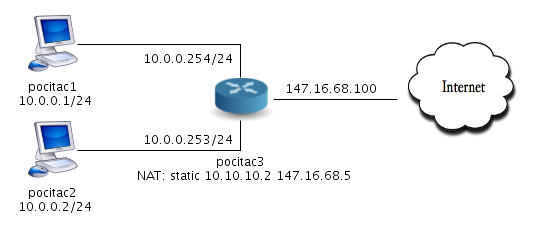
\includegraphics[width=12cm]{figures/nat1}
\caption{Statický překlad adres}
\label{fig:nat1}
\end{center}
\end{figure}

\newpage


\subsubsection{Dynamický NAT a overloading}
Dynamický překlad adres je velmi podobný statickému s tím rozdílem, že se pravidla generují dynamicky. Je pouze přiřazen pool IP adres\footnote{pool je doslova zásoba či rezerva}, ze kterého se přiřazují adresy (s portem) při překladu. Navíc lze omezit adresy sítí, které se mají překládat (příkaz \verb|access-list|).

Overloading je spíše podmnožina dynamického NATu, kde je povoleno přiřazovat jednu IP adresu více počítačům. Pakety od různých počítačů jsou pak odlišeny jiným portem.

Dynamický překlad probíhá tak, že se nejdříve zkontrolují access-listy, zda se má vůbec překládat. Když IP adresa spadá do access-listu, tak se vezme volná IP adresa (při metodě overloading může být vybrána jedna adresa vícekrát) z poolu, který je k access-listu přiřazen. Touto vybranou IP adresou počítač přepíše zdrojovou adresu příchozího paketu a vytvoří dynamický záznam do NAT tabulky. Zpětná překlad je jednodušší. Počítač vybere dynamický záznam, přepíše cílovou adresu a předá paket směrovacím pravidlům.

\paragraph{IOS příkazy}
Přidat pool adres lze příkazem:
\begin{verbatim}
ip nat pool <POOL_JMENO> <IP_START> <IP_KONEC> prefix <PREFIX>
POOL_JMENO - název poolu IP adres
IP_START - adresa, od které se budou adresy generovat
IP_KONEC - adresa, do které se budou adresy generovat
PREFIX - maska poolu v počtu jedničkových bitů
\end{verbatim} 

Přístupový list pro omezení překladu adres se přidá přes příkaz:
\begin{verbatim}
access-list <CISLO> permit <IP> <WILDCARD>
CISLO - identifikátor access-listu
IP - adresa sítě povolených IP adres
WILDCARD - maska ve tvaru wildcard (maska = broadcast - wildcard)
\end{verbatim}

Pro přiřazení poolu k access-listu se provadí pomocí příkazu:
\begin{verbatim}
ip nat inside source list <ACCESS-LIST> pool <POOL> overload?
ACCESS-LIST - identifikátor access-listu
POOL - jméno poolu
overload - nepovinná volba pro overloading
\end{verbatim} 

%------------------------------------------------------------------------------

\subsection{Návrh a implementace NATu}

\subsubsection{Návrh}
Každý počítač bude mít vlastní NAT tabulku. Ta bude složená ze seznamu \verb|NATzaznam|. Dále NAT tabulka bude potřebovat seznam soukromých rozhraní a odkaz na jedno veřejné. Bude také potřeba si držet číslo aktuálního access-listu, poolu a stav příznaku overloading. Vše ilustruje obrázek \ref{fig:nat_navrh1}.

\begin{figure}[h]
\begin{center}
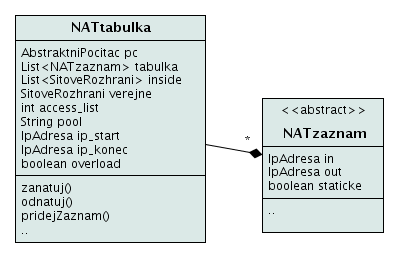
\includegraphics[width=9cm]{figures/nat_navrh1}
\caption{Návrh překladu adres č.1}
\label{fig:nat_navrh1}
\end{center}
\end{figure}

\subsubsection{Implementace}
Při implementaci NAT tabulky vyplula na povrch chyba v návrhu. Návrh počítal s tím, že může být pouze jeden pool a jeden access-list. Skutečné cisco si ale pamatuje bez problému i stovky těchto příkazů. Z tohoto důvodu jsem musel původní návrh přizpůsobit. Přidal jsem několik dalších datových struktur, které mi v pozdější fázi velmi usnadnili manipulaci s NAT tabulkou. Na obrázku \ref{fig:nat_navrh2} je znázorněn nový návrh.

\begin{figure}[b]
\begin{center}
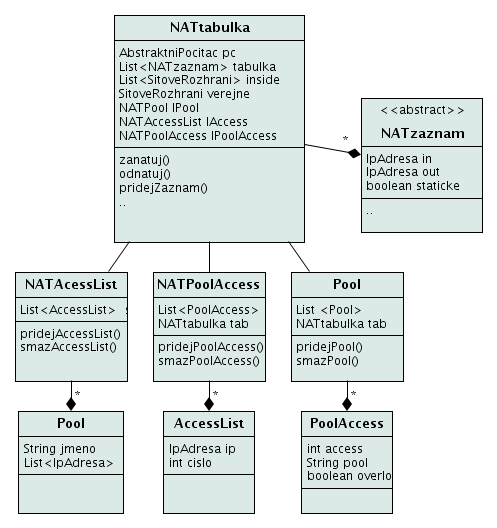
\includegraphics[width=12cm]{figures/nat_navrh2}
\caption{Návrh překladu adres č.2 - finální}
\label{fig:nat_navrh2}
\end{center}
\end{figure}

\paragraph{Postup překladu adres}
Podrobný postup překladu adres na skutečném ciscu je zde \cite{cisco:postup}.

\subparagraph{Směr ven}
Když přijde paket do počítače, tak se nejdříve provede reverzní překlad\footnote{Reverzní překlad by v češtině nejlépe vystihoval výraz \uv{\textit{odnatování}}.}. Po té počítač dle routovací tabulky rozhodne, na které rozhraní paket odešle. Pak přichází na řadu samotný akt překladu adres. Chování NATu je řízeno několika pravidly:

\begin{itemize}
\item Když příchozí rozhraní\footnote{Rozhraní, pomocí kterého byl paket do počítače přijat.} není označeno jako soukromé\footnote{V Cisco IOSu pomocí příkazu \uv{ip nat inside}.} nebo odchozí rozhraní není označeno jako veřejné\footnote{Veřejné rozhraní je označeno \uv{ip nat outside}.}, tak se paket přepošle dál bez překladu adres.

\item Pokud lze nalézt statické pravidlo, které by odpovídalo zdrojové adrese, tak se přeloží zdrojová adresa dle tohoto pravida.

\item Když není nalezen žádný access-list, který by odpovídal zdrojové adrese, tak se paket přepošle bez překladu.

\item Když zdrojová adresa paketu spadá do access-listu, ke kterému není přiřazen žádný pool, tak se pošle zpět odesílateli \verb|Destination Host Unreacheble|.

\item Když v IP poolu, který je přiřazen k odpovídajícímu access-listu, dojdou volné IP adresy, tak se pošle zpět odesílateli \verb|Destination Host Unreacheble|.

\item V ostatních případech se provede překlad adres:
    \begin{enumerate}
    \item Zkusí se nalézt odpovídající dynamické pravidlo. V případě nenalezení viz následující bod.
    \item Vygeneruje se nová IP adresa z poolu a vloží se takto vytvořený záznam do NAT tabulky.
    \end{enumerate}
\end{itemize}

Vše je lépe znázorněno na vývojovém diagramu \ref{fig:nat_decision}.

\begin{figure}[b]
\begin{center}
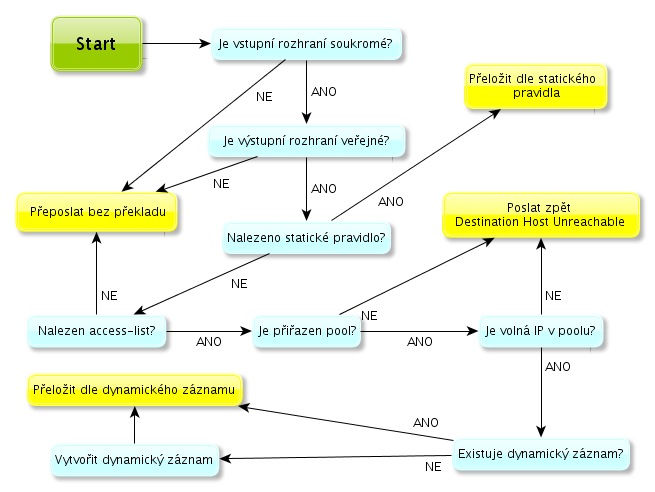
\includegraphics[width=16cm]{figures/nat_decision}
\caption{Vývojový diagram překladu adres}
\label{fig:nat_decision}
\end{center}
\end{figure}

% routovani
% zanatovava se kdyz je prichozi soukrome, kdyz odchozi je verejne
% musit patrit do access-listu (kdyz nepatri, tak jen preposlat bez odnatovani)
% k nemu musi byt prirazen pool (kdyz neni tak se posila zpet DHU)
% kdyz neni volna IP (už došli), tak se posle zpet DHU
% IP je v a-listech && je volná IP tak se natuje:
%     pokud je stat. prav. tak se zanatuje
%     pokud je dyn. prav. tak se zanatuje
%     kdyz nic, tak se vygeneruje novy dyn. zaznam a prida se do tabulky
%     prelozi je zdrojova a odesle do vnejsi site



\subparagraph{Směr dovnitř - reverzní překlad}

Reverzní překlad je mnohem jednodušší záležitost. Příchozí paket čekají tyto pravidla:
\begin{enumerate}
  \item Nejdříve se zkontroluje, zda paket přišel přes veřejné rozhraní. Když je vstupní rozhraní jiné než neřejné, tak se reverzní překlad neprovede.

  \item Pak se prohledají statická pravidla, zda nějaké odpovídá (včetně portu) cílové adrese paketu. Pokud odpovídá, tak se provede reverzní překlad.

  \item Když se nenajde ani žádný dynamický záznam, tak se cílová adresa paketu překládat nebude a paket zůstane beze změny.
\end{enumerate}


\subsubsection*{}
Z obou směrů překladu vyplývá, že statická pravidla mají přednost před dynamickými záznamy. Při testování NATu na školních ciscách jsem zjistil, že cisca zapomínají všechny dynamické záznamy starší cca 10 vteřin. Tato vlastnost byla dodatečně implementována i do této aplikace. Více informací o konfiguraci statického a dynamického NATu zároveň je na stránkách Cisco Systems\cite{cisco:snat_dnat}




% odnatovava se kdyz je nastaveno verejne rozhr. a kdyz to taky z nej prislo
% juk do tabulky - staticke, pak dyn.
% pak smerovani
% odeslani do vnitrni site






% \section{Načítání ze souboru}
\subsection{Zpracování parametrů}
Po spuštění startovacího skriptu \verb|start_server.sh| se nejdříve zpracují všechny parametry. Když je nalezen parametr \verb|-n|, tak se načítá z konfiguračního souboru pouze kostra sítě s počítačema a rozhraníma bez jejich nastavení. Pozice tohoto parametru není důležitá, systém nejprve detekuje přítomnost tohoto parametr a pak už ho vůbec neřeší. Další parametr je název konfiguračního souboru, ten může být zadán bez koncovky \verb|.xml|, nejdříve se zkusí načíst soubor bez koncovky a když takový soubor není, tak se načte soubor s koncovkou. Třetím parametrem je port, od kterého budou poslouchat jednotlivé počítače. Port je nepovinný, výchozí volba je port 4000. Když je daný port obsazený, tak se program ukončí z chybovou hláškou.

%------------------------------------------------------------------------------

\subsection{Konfigurační soubor}
Nejdříve bylo nutno rozhodnout podobu výsledného konfiguračního souboru. Existuje několik možností, např.:
\begin{itemize}
 \item javovské \verb|Properties| ve stylu \uv{proměnná = hodnota}, moc se nehodí na velmi členité struktury
\begin{verbatim}
compile.on.save=false
do.depend=false
do.jar=true
javac.debug=true
\end{verbatim} 

 \item podoba konfiguračních souborů KDE\footnote{K Desktop Environment je desktopové prostředí pro Linux a další unixové operační systémy.}, kde jednotlivé sekce jsou odděleny jménem v hranatých závorkách
\begin{verbatim}
[Xdmcp]
Enable=false
[Shutdown]
# Default is "/sbin/halt"
HaltCmd=/sbin/shutdown
\end{verbatim} 

 \item XML\footnote{Extensible Markup Language je rozšiřitelný značkovací jazyk} soubor, který umožňuje libovolnou strukturu
\end{itemize}

Já jsem si vybral technologii XML pro jeho robustnost a velmi dobrou čitelnost.

Načítání z XML souboru lze udělat minimálně dvěma způsoby: Vzít cizí knihovnu, která tuto funkcionalitu zajišťuje, nebo vytvořit vlastní třídu. Obě možnosti mají své výhody i nevýhody. Cizí knihovna by mohla být téměř bez práce a pravděpodobně by podporovala i zpětné ukládání. Na druhou stranu by byla malá možnost ovlivnění výsledného výstupu a bylo by vše na té knihovně závislé. Navíc s novými verzemi by se mohla měnit i její funkčnost. Znamenalo by to také instalaci této knihovny na uživatelských počítačích. Z těchto důvodů jsem zvolil druhou variantu: vlastní implementace zpracování XML. 

%------------------------------------------------------------------------------

\subsection{Implementace SAX handleru}
Zpracovat XML lze přes technologii DOM\footnote{Document Object Model} a SAX\footnote{Simple API for XML}. Já se rozhodl pro SAX z těchto důvodů:
\begin{itemize}
 \item jednorázové sekvenční čtení - vyšší rychlost
 \item menší paměťová náročnost
 \item oproti DOMu i několikrát rychlejší, což u velmi rozlehlé síťě by mohlo být znatelné
\end{itemize}

Můj \verb|SAXHandler| tvoří tři části: samotné načítání, datová struktura pro počítač a vytváření virtuálního počítače.

\subsubsection{Načítání}
\verb|ContentHandler| vyhazuje události při zpracování XML souboru. \verb|SAXHandler| musí tyto události odchytávat a pokud je to událost, která nás zajímá, tak se zpracuje tj. uloží do datové sktruktury. Musí být implementovány metody na zpracování začátku elementu, konce elementu, znaková data a konce dokumentu. Po načtení konce elementu se vytvoří virtuální síť počítačů. Pro správnou funkci \verb|SAXHandler| je důležité mít ve složce s konfiguračními soubory také soubor DTD\footnote{Document Type Definition}, který definuje strukturu XML dokumentu.

\subsubsection{Datová struktura}
Pro ukládání informací slouží datová struktura \verb|PocitacBuilder|, která si drží veškeré informace načtené z XML souboru o jednom počítači:
\begin{itemize}
 \item jméno a typ počítače
 \item nastavení rozhraní - jméno, adresa, maska, stav
 \item routovací tabulka - výčet záznamů
 \item ip\_forward - pro potřeby Linuxu
 \item překlad adres - pooly adres, access-listy, přiřazení access-listů k poolům, statické záznamy
\end{itemize}

Pak je tu ještě sekundární struktura pro uložení kabelů k jednotlivým počítačům.

\subsubsection{Vytváření virtuálních počítačů}
Po vyhození události konec souboru se začnou vyrábět virtuální počítače. Pokud byl použit parametr \verb|-n|, tak se nejdříve smažou nastavení, která nemají být načtena. Po té se postupně budou načítat (a kontrolovat) všechny uložené nastavení. V zásadě lze říci, že když systém narazí na neplatná data v konfiguračním souboru, tak vypíše chybovou hlášku na standardní chybový výstup. Pokud je to chyba zásadní, tak se vyhodí výjimka, vypíše hláška a celý server se ukončí, protože nemůže pokračovat v další činnosti. Slovem zásadní je myšleno např. chybějící jméno rozhraní (kabely v XML jsou napojeny přes jména rozhraní), natažená kabeláž a opakující se jména počítačů či rozhraní na jednom počítači. Kabely jsou natolik klíčovou věcí, že uživatele upozorní na chybu pádem programu s výpisem, co je špatně. 

Takto vypadá příklad konfiguračního souboru:
\begin{verbatim}
<pocitac jmeno="cisco1" typ="cisco">
  <rozhrani>
    <jmeno>FastEthernet0/0</jmeno>
    <ip>192.168.1.254</ip>
    <maska>255.255.255.0</maska>
    <mac>00:0b:0c:0d:0a:01</mac>
    <nahozene>true</nahozene>
    <nat>soukrome</nat>
  </rozhrani>
...
\end{verbatim} 

%------------------------------------------------------------------------------

\section{Ukládání do souboru}
Abstraktní \verb|ParserPrikazu| obsahuje metodu, do které jsou vloženy všechny společné příkazy. V současné době je tam pouze příkaz \verb|uloz| alias \verb|save|. Uživatel může použít jakoukoliv variantu dle libosti. Při zavolání tohoto příkazu bez parametru se bude ukládat do stejného souboru, ze kterého se při staru aplikace načítalo. Nebo může uživatel specifikovat jméno souboru (včetně cesty), do kterého se má aktuální konfigurace uložit. 

Ukládání do souboru je realizováno čistě textově, tzn. vše se posílá přes \verb|BufferedWriter| bez použítí externích knihoven. Pro usnadnění práce jsem si napsal několik pomocných metod, kde např. pro uložení MAC adresy do XML stačí zavolat \\\verb|zapisElement("mac", rozhrani.macAdresa)|. Velmi užitečná metoda je také \verb|vratElement|, která postaví element s daným jménem a obsahem:
\begin{verbatim}
private String vratElement(String jmeno, String obsah) {
  if (obsah == null) {
    obsah = "";
  }
  return "<" + jmeno + ">" + obsah + "</" + jmeno + ">\n";
}
\end{verbatim} 


Výhodou tohoto řešení je maximální kontrola nad výstupem příkazu a jednudochost implementace. Mezi nevýhody bych uvedl hlavně změnu v datových strukturách. Když by bylo potřeba připsat novou volbu, která by se měla ukládat do XML souboru, tak musíme přidat pravidla pro načítání z XML v \verb|SAXHandler| a navíc zde ukládání.




% atd...

%*****************************************************************************

% Výsledná struktura vaší práce a~názvy a~rozsahy jednotlivých kapitol se samozřejmě budou lišit podle typu práce a~podle
% konkrétní povahy zpracovávaného tématu. Níže uvedená struktura práce odpovídá \textit{práci implementační}, viz
% \cite{infodp} respektive \cite{infobp}. 

%*****************************************************************************
\chapter{Testování}

\begin{itemize}
 \item Způsob, průběh a~výsledky testování.
 \item Srovnání s~existujícími řešeními, pokud jsou známy.
\end{itemize} 


%*****************************************************************************
\chapter{Závěr}
\section{Možnosti vylepšení}

\begin{itemize}
\item Zhodnocení splnění cílů DP/BP a~vlastního přínosu práce (při formulaci je třeba vzít v~potaz zadání práce).
\item Diskuse dalšího možného pokračování práce.
\begin{itemize}
\item graficke klikatko pro tvorbu XML konfiguraku
\item tcpdump
\item switche
\item napojeni na realnou sit
\item zpracovani signalu Ctrl+C, Ctrl+Z (-> vlastni klient, kouzlo telnetu je pak pryc)
\end{itemize} 


\end{itemize} 

%*****************************************************************************
% Seznam literatury je v samostatnem souboru reference.bib. Ten
% upravte dle vlastnich potreb, potom zpracujte (a do textu
% zapracujte) pomoci prikazu bibtex a nasledne pdflatex (nebo
% latex). Druhy z nich alespon 2x, aby se poresily odkazy.

% originally following specification for bibliography formating was used
%\bibliographystyle{abbrv}

% Here is an improvment by Petr Dlouhy (April 2010).
% It is mainly for supervisors who expect Czech fomrating rules for references
% Additional feature is live url addresses to sources from your pdf file
% It requires the file csplainnat.bst (included in this sample zipfile).

\bibliographystyle{csplainnat}

%bibliographystyle{plain}
%\bibliographystyle{psc}
{
%JZ: 11.12.2008 Kdo chce mit v techto ukazkovych odkazech take odkaz na CSTeX:
\def\CS{$\cal C\kern-0.1667em\lower.5ex\hbox{$\cal S$}\kern-0.075em $}
\bibliography{reference}
}

% M. Dušek radi:
%\bibliographystyle{alpha}
% kdy citace ma tvar [AutorRok] (napriklad [Cook97]). Sice to asi neni  podle ceske normy (BTW BibTeX stejne neodpovida
ceske norme), ale je to nejprehlednejsi.
% 3.5.2009 JZ polemizuje: BibTeX neobvinujte, napiste a poskytnete nam styl (.bst) splnujici citacni normu CSN/ISO.

%*****************************************************************************
%*****************************************************************************
\appendix

\chapter{Testování zaplnění stránky a~odsazení odstavců}
\textbf{\large Tato příloha nebude součástí vaší práce. 
Slouží pouze jako příklad formátování textu.}

\section*{}
Určitě existuje nějaká pěkná latinská věta, která se k~tomuhle testování používá, ale co mají dělat ti, kteří se nikdy
latinsky neučili? Určitě existuje nějaká pěkná latinská věta, která se k~tomuhle testování používá, ale co mají dělat
ti, kteří se nikdy latinsky neučili? Určitě existuje nějaká pěkná latinská věta, která se k~tomuhle testování používá,
ale co mají dělat ti, kteří se nikdy latinsky neučili?

Určitě existuje nějaká pěkná latinská věta, která se k~tomuhle testování používá, ale co mají dělat ti, kteří se nikdy
latinsky neučili? Určitě existuje nějaká pěkná latinská věta, která se k~tomuhle testování používá, ale co mají dělat
ti, kteří se nikdy latinsky neučili? Určitě existuje nějaká pěkná latinská věta, která se k~tomuhle testování používá,
ale co mají dělat ti, kteří se nikdy latinsky neučili?

Určitě existuje nějaká pěkná latinská věta, která se k~tomuhle testování používá, ale co mají dělat ti, kteří se nikdy
latinsky neučili? Určitě existuje nějaká pěkná latinská věta, která se k~tomuhle testování používá, ale co mají dělat
ti, kteří se nikdy latinsky neučili? Určitě existuje nějaká pěkná latinská věta, která se k~tomuhle testování používá,
ale co mají dělat ti, kteří se nikdy latinsky neučili?

Určitě existuje nějaká pěkná latinská věta, která se k~tomuhle testování používá, ale co mají dělat ti, kteří se nikdy
latinsky neučili? Určitě existuje nějaká pěkná latinská věta, která se k~tomuhle testování používá, ale co mají dělat
ti, kteří se nikdy latinsky neučili? Určitě existuje nějaká pěkná latinská věta, která se k~tomuhle testování používá,
ale co mají dělat ti, kteří se nikdy latinsky neučili? Určitě existuje nějaká pěkná latinská věta, která se k~tomuhle
testování používá, ale co mají dělat ti, kteří se nikdy latinsky neučili? Určitě existuje nějaká pěkná latinská věta,
která se k~tomuhle testování používá, ale co mají dělat ti, kteří se nikdy latinsky neučili? Určitě existuje nějaká
pěkná latinská věta, která se k~tomuhle testování používá, ale co mají dělat ti, kteří se nikdy latinsky neučili?

Určitě existuje nějaká pěkná latinská věta, která se k~tomuhle testování používá, ale co mají dělat ti, kteří se nikdy
latinsky neučili? Určitě existuje nějaká pěkná latinská věta, která se k~tomuhle testování používá, ale co mají dělat
ti, kteří se nikdy latinsky neučili?

Určitě existuje nějaká pěkná latinská věta, která se k~tomuhle testování používá, ale co mají dělat ti, kteří se nikdy
latinsky neučili? Určitě existuje nějaká pěkná latinská věta, která se k~tomuhle testování používá, ale co mají dělat
ti, kteří se nikdy latinsky neučili? Určitě existuje nějaká pěkná latinská věta, která se k~tomuhle testování používá,
ale co mají dělat ti, kteří se nikdy latinsky neučili? Určitě existuje nějaká pěkná latinská věta, která se k~tomuhle
testování používá, ale co mají dělat ti, kteří se nikdy latinsky neučili? Určitě existuje nějaká pěkná latinská věta,
která se k~tomuhle testování používá, ale co mají dělat ti, kteří se nikdy latinsky neučili?

Určitě existuje nějaká pěkná latinská věta, která se k~tomuhle testování používá, ale co mají dělat ti, kteří se nikdy
latinsky neučili? Určitě existuje nějaká pěkná latinská věta, která se k~tomuhle testování používá, ale co mají dělat
ti, kteří se nikdy latinsky neučili? Určitě existuje nějaká pěkná latinská věta, která se k~tomuhle testování používá,
ale co mají dělat ti, kteří se nikdy latinsky neučili? Určitě existuje nějaká pěkná latinská věta, která se k~tomuhle
testování používá, ale co mají dělat ti, kteří se nikdy latinsky neučili? Určitě existuje nějaká pěkná latinská věta,
která se k~tomuhle testování používá, ale co mají dělat ti, kteří se nikdy latinsky neučili?

Určitě existuje nějaká pěkná latinská věta, která se k~tomuhle testování používá, ale co mají dělat ti, kteří se nikdy
latinsky neučili? Určitě existuje nějaká pěkná latinská věta, která se k~tomuhle testování používá, ale co mají dělat
ti, kteří se nikdy latinsky neučili? Určitě existuje nějaká pěkná latinská věta, která se k~tomuhle testování používá,
ale co mají dělat ti, kteří se nikdy latinsky neučili? Určitě existuje nějaká pěkná latinská věta, která se k~tomuhle
testování používá, ale co mají dělat ti, kteří se nikdy latinsky neučili? Určitě existuje nějaká pěkná latinská věta,
která se k~tomuhle testování používá, ale co mají dělat ti, kteří se nikdy latinsky neučili?

Určitě existuje nějaká pěkná latinská věta, která se k~tomuhle testování používá, ale co mají dělat ti, kteří se nikdy
latinsky neučili? Určitě existuje nějaká pěkná latinská věta, která se k~tomuhle testování používá, ale co mají dělat
ti, kteří se nikdy latinsky neučili? Určitě existuje nějaká pěkná latinská věta, která se k~tomuhle testování používá,
ale co mají dělat ti, kteří se nikdy latinsky neučili? Určitě existuje nějaká pěkná latinská věta, která se k~tomuhle
testování používá, ale co mají dělat ti, kteří se nikdy latinsky neučili? Určitě existuje nějaká pěkná latinská věta,
která se k~tomuhle testování používá, ale co mají dělat ti, kteří se nikdy latinsky neučili?

Určitě existuje nějaká pěkná latinská věta, která se k~tomuhle testování používá, ale co mají dělat ti, kteří se nikdy
latinsky neučili? Určitě existuje nějaká pěkná latinská věta, která se k~tomuhle testování používá, ale co mají dělat
ti, kteří se nikdy latinsky neučili? Určitě existuje nějaká pěkná latinská věta, která se k~tomuhle testování používá,
ale co mají dělat ti, kteří se nikdy latinsky neučili? Určitě existuje nějaká pěkná latinská věta, která se k~tomuhle
testování používá, ale co mají dělat ti, kteří se nikdy latinsky neučili? Určitě existuje nějaká pěkná latinská věta,
která se k~tomuhle testování používá, ale co mají dělat ti, kteří se nikdy latinsky neučili?

Určitě existuje nějaká pěkná latinská věta, která se k~tomuhle testování používá, ale co mají dělat ti, kteří se nikdy
latinsky neučili? Určitě existuje nějaká pěkná latinská věta, která se k~tomuhle testování používá, ale co mají dělat
ti, kteří se nikdy latinsky neučili? Určitě existuje nějaká pěkná latinská věta, která se k~tomuhle testování používá,
ale co mají dělat ti, kteří se nikdy latinsky neučili? Určitě existuje nějaká pěkná latinská věta, která se k~tomuhle
testování používá, ale co mají dělat ti, kteří se nikdy latinsky neučili? Určitě existuje nějaká pěkná latinská věta,
která se k~tomuhle testování používá, ale co mají dělat ti, kteří se nikdy latinsky neučili?

Určitě existuje nějaká pěkná latinská věta, která se k~tomuhle testování používá, ale co mají dělat ti, kteří se nikdy
latinsky neučili? Určitě existuje nějaká pěkná latinská věta, která se k~tomuhle testování používá, ale co mají dělat
ti, kteří se nikdy latinsky neučili? Určitě existuje nějaká pěkná latinská věta, která se k~tomuhle testování používá,
ale co mají dělat ti, kteří se nikdy latinsky neučili? Určitě existuje nějaká pěkná latinská věta, která se k~tomuhle
testování používá, ale co mají dělat ti, kteří se nikdy latinsky neučili? Určitě existuje nějaká pěkná latinská věta,
která se k~tomuhle testování používá, ale co mají dělat ti, kteří se nikdy latinsky neučili?

Určitě existuje nějaká pěkná latinská věta, která se k~tomuhle testování používá, ale co mají dělat ti, kteří se nikdy
latinsky neučili? Určitě existuje nějaká pěkná latinská věta, která se k~tomuhle testování používá, ale co mají dělat
ti, kteří se nikdy latinsky neučili? Určitě existuje nějaká pěkná latinská věta, která se k~tomuhle testování používá,
ale co mají dělat ti, kteří se nikdy latinsky neučili? Určitě existuje nějaká pěkná latinská věta, která se k~tomuhle
testování používá, ale co mají dělat ti, kteří se nikdy latinsky neučili? Určitě existuje nějaká pěkná latinská věta,
která se k~tomuhle testování používá, ale co mají dělat ti, kteří se nikdy latinsky neučili?

Určitě existuje nějaká pěkná latinská věta, která se k~tomuhle testování používá, ale co mají dělat ti, kteří se nikdy
latinsky neučili? Určitě existuje nějaká pěkná latinská věta, která se k~tomuhle testování používá, ale co mají dělat
ti, kteří se nikdy latinsky neučili? Určitě existuje nějaká pěkná latinská věta, která se k~tomuhle testování používá,
ale co mají dělat ti, kteří se nikdy latinsky neučili? Určitě existuje nějaká pěkná latinská věta, která se k~tomuhle
testování používá, ale co mají dělat ti, kteří se nikdy latinsky neučili? Určitě existuje nějaká pěkná latinská věta,
která se k~tomuhle testování používá, ale co mají dělat ti, kteří se nikdy latinsky neučili?

Určitě existuje nějaká pěkná latinská věta, která se k~tomuhle testování používá, ale co mají dělat ti, kteří se nikdy
latinsky neučili? Určitě existuje nějaká pěkná latinská věta, která se k~tomuhle testování používá, ale co mají dělat
ti, kteří se nikdy latinsky neučili? Určitě existuje nějaká pěkná latinská věta, která se k~tomuhle testování používá,
ale co mají dělat ti, kteří se nikdy latinsky neučili? Určitě existuje nějaká pěkná latinská věta, která se k~tomuhle
testování používá, ale co mají dělat ti, kteří se nikdy latinsky neučili? Určitě existuje nějaká pěkná latinská věta,
která se k~tomuhle testování používá, ale co mají dělat ti, kteří se nikdy latinsky neučili?

Určitě existuje nějaká pěkná latinská věta, která se k~tomuhle testování používá, ale co mají dělat ti, kteří se nikdy
latinsky neučili? Určitě existuje nějaká pěkná latinská věta, která se k~tomuhle testování používá, ale co mají dělat
ti, kteří se nikdy latinsky neučili? Určitě existuje nějaká pěkná latinská věta, která se k~tomuhle testování používá,
ale co mají dělat ti, kteří se nikdy latinsky neučili? Určitě existuje nějaká pěkná latinská věta, která se k~tomuhle
testování používá, ale co mají dělat ti, kteří se nikdy latinsky neučili? Určitě existuje nějaká pěkná latinská věta,
která se k~tomuhle testování používá, ale co mají dělat ti, kteří se nikdy latinsky neučili?

Určitě existuje nějaká pěkná latinská věta, která se k~tomuhle testování používá, ale co mají dělat ti, kteří se nikdy
latinsky neučili? Určitě existuje nějaká pěkná latinská věta, která se k~tomuhle testování používá, ale co mají dělat
ti, kteří se nikdy latinsky neučili? Určitě existuje nějaká pěkná latinská věta, která se k~tomuhle testování používá,
ale co mají dělat ti, kteří se nikdy latinsky neučili? Určitě existuje nějaká pěkná latinská věta, která se k~tomuhle
testování používá, ale co mají dělat ti, kteří se nikdy latinsky neučili? Určitě existuje nějaká pěkná latinská věta,
která se k~tomuhle testování používá, ale co mají dělat ti, kteří se nikdy latinsky neučili?

Určitě existuje nějaká pěkná latinská věta, která se k~tomuhle testování používá, ale co mají dělat ti, kteří se nikdy
latinsky neučili? Určitě existuje nějaká pěkná latinská věta, která se k~tomuhle testování používá, ale co mají dělat
ti, kteří se nikdy latinsky neučili? Určitě existuje nějaká pěkná latinská věta, která se k~tomuhle testování používá,
ale co mají dělat ti, kteří se nikdy latinsky neučili? Určitě existuje nějaká pěkná latinská věta, která se k~tomuhle
testování používá, ale co mají dělat ti, kteří se nikdy latinsky neučili? Určitě existuje nějaká pěkná latinská věta,
která se k~tomuhle testování používá, ale co mají dělat ti, kteří se nikdy latinsky neučili?

Určitě existuje nějaká pěkná latinská věta, která se k~tomuhle testování používá, ale co mají dělat ti, kteří se nikdy
latinsky neučili? Určitě existuje nějaká pěkná latinská věta, která se k~tomuhle testování používá, ale co mají dělat
ti, kteří se nikdy latinsky neučili? Určitě existuje nějaká pěkná latinská věta, která se k~tomuhle testování používá,
ale co mají dělat ti, kteří se nikdy latinsky neučili? Určitě existuje nějaká pěkná latinská věta, která se k~tomuhle
testování používá, ale co mají dělat ti, kteří se nikdy latinsky neučili? Určitě existuje nějaká pěkná latinská věta,
která se k~tomuhle testování používá, ale co mají dělat ti, kteří se nikdy latinsky neučili?

Určitě existuje nějaká pěkná latinská věta, která se k~tomuhle testování používá, ale co mají dělat ti, kteří se nikdy
latinsky neučili? Určitě existuje nějaká pěkná latinská věta, která se k~tomuhle testování používá, ale co mají dělat
ti, kteří se nikdy latinsky neučili? Určitě existuje nějaká pěkná latinská věta, která se k~tomuhle testování používá,
ale co mají dělat ti, kteří se nikdy latinsky neučili? Určitě existuje nějaká pěkná latinská věta, která se k~tomuhle
testování používá, ale co mají dělat ti, kteří se nikdy latinsky neučili? Určitě existuje nějaká pěkná latinská věta,
která se k~tomuhle testování používá, ale co mají dělat ti, kteří se nikdy latinsky neučili?

%*****************************************************************************

\chapter{Pokyny a~návody k~formátování textu práce}
\textbf{\large Tato příloha samozřejmě nebude součástí vaší práce. Slouží pouze jako příklad formátování textu.}

Používat se dají všechny příkazy systému \LaTeX. Existuje velké množství volně přístupné dokumentace, tutoriálů,
příruček a~dalších materiálů v~elektronické podobě. Výchozím bodem, kromě Googlu, může být stránka CSTUG (Czech Tech
Users Group) \cite{CSTUG}. Tam najdete odkazy na další materiály.  Vetšinou dostačující a~přehledně organizovanou
elektronikou dokumentaci najdete například na \cite{latexdocweb} nebo \cite{latexwiki}.

Existují i~různé nadstavby nad systémy \TeX{} a~\LaTeX, které výrazně usnadní psaní textu zejména začátečníkům. Velmi
rozšířený v~Linuxovém prostředí je systém Kile.


\section{Vkládání obrázků}
Obrázky se umísťují do plovoucího prostředí \verb|figure|. Každý obrázek by měl obsahovat \textbf{název}
(\verb|\caption|) a~\textbf{návěští} (\verb|\label|). Použití příkazu pro vložení obrázku \\\verb|\includegraphics| je
podmíněno aktivací (načtením) balíku graphicx příkazem\\ \verb|\usepackage{graphicx}|.

Budete-li zdrojový text zpracovávat pomocí programu \verb|pdflatex|, očekávají se obrázky s~příponou
\verb|*.pdf|\footnote{pdflatex umí také formáty PNG a~JPG.}, použijete-li k~formátování \verb|latex|, očekávají se
obrázky s~příponou \verb|*.eps|.\footnote{Vzájemnou konverzi mezi snad všemi typy obrazku včetně změn vekostí a~dalších
vymožeností vám může zajistit balík ImageMagic  (http://www.imagemagick.org/script/index.php). Je dostupný pod Linuxem,
Mac OS i~MS Windows. Důležité jsou zejména příkazy convert a~identify.}


\begin{figure}[ht]
\begin{center}

\includegraphics[width=5cm]{figures/LogoCVUT}
\caption{Popiska obrázku}
\label{fig:logo}
\end{center}
\end{figure}

Příklad vložení obrázku:
\begin{verbatim}
\begin{figure}[h]
\begin{center}

\includegraphics[width=5cm]{figures/LogoCVUT}
\caption{Popiska obrazku}
\label{fig:logo}
\end{center}
\end{figure}
\end{verbatim}

\section{Kreslení obrázků}
Zřejmě každý z~vás má nějaký oblíbený nástroj pro tvorbu obrázků. Jde jen o~to, abyste dokázali obrázek uložit
v~požadovaném formátu nebo jej do něj konvertovat (viz předchozí kapitola). Je zřejmě vhodné kreslit obrázky vektorově.
Celkem oblíbený, na ovládání celkem jednoduchý a~přitom dostatečně mocný je například program Inkscape.

Zde stojí za to upozornit na kreslící programe Ipe \cite{ipe}, který dokáže do obrázku vkládat komentáře přímo
v~latexovském formátu (vzroce, stejné fonty atd.). Podobné věci umí na Linuxové platformě nástroj Xfig. 

Za pozornost ještě stojí schopnost editoru Ipe importovat obrázek (jpg nebo bitmap) a~krelit do něj latexovské popisky
a~komentáře. Výsledek pak umí exportovat přímo do pdf.


\section{Tabulky}
Existuje více způsobů, jak sázet tabulky. Například je možno použít prostředí \verb|table|, které je velmi podobné
prostředí \verb|figure|. 

\begin{table}
\begin{center}
\begin{tabular}{|c|l|l|}
\hline
\textbf{DTD} & \textbf{construction} & \textbf{elimination} \\
\hline
$\mid$ & \verb+in1|A|B a:sum A B+ & \verb+case([_:A]a)([_:B]a)ab:A+\\
&\verb+in1|A|B b:sum A B+ & \verb+case([_:A]b)([_:B]b)ba:B+\\
\hline
$+$&\verb+do_reg:A -> reg A+&\verb+undo_reg:reg A -> A+\\
\hline
$*,?$& the same like $\mid$ and $+$ & the same like $\mid$ and $+$\\
& with \verb+emtpy_el:empty+ & with \verb+emtpy_el:empty+\\
\hline
R(a,b) & \verb+make_R:A->B->R+ & \verb+a: R -> A+\\
 & & \verb+b: R -> B+\\
\hline
\end{tabular}
\end{center}
\caption{Ukázka tabulky}
\label{tab:tab1}
\end{table}

Zdrojový text tabulky \ref{tab:tab1} vypadá takto:
\begin{verbatim}
\begin{table}
\begin{center}
\begin{tabular}{|c|l|l|}
\hline
\textbf{DTD} & \textbf{construction} & \textbf{elimination} \\
\hline
$\mid$ & \verb+in1|A|B a:sum A B+ & \verb+case([_:A]a)([_:B]a)ab:A+\\
&\verb+in1|A|B b:sum A B+ & \verb+case([_:A]b)([_:B]b)ba:B+\\
\hline
$+$&\verb+do_reg:A -> reg A+&\verb+undo_reg:reg A -> A+\\
\hline
$*,?$& the same like $\mid$ and $+$ & the same like $\mid$ and $+$\\
& with \verb+emtpy_el:empty+ & with \verb+emtpy_el:empty+\\
\hline
R(a,b) & \verb+make_R:A->B->R+ & \verb+a: R -> A+\\
 & & \verb+b: R -> B+\\
\hline
\end{tabular}
\end{center}
\caption{Ukázka tabulky}
\label{tab:tab1}
\end{table}
\begin{table}
\end{verbatim}

\section{Odkazy v~textu}
\subsection{Odkazy na literaturu}
Jsou realizovány příkazem \verb|\cite{odkaz}|. 

Seznam literatury je dobré zapsat do samostatného souboru a~ten pak zpracovat programem bibtex (viz soubor
\verb|reference.bib|). Zdrojový soubor pro \verb|bibtex| vypadá například takto:
\begin{verbatim}
@Article{Chen01,
  author  = "Yong-Sheng Chen and Yi-Ping Hung and Chiou-Shann Fuh",
  title   = "Fast Block Matching Algorithm Based on 
             the Winner-Update Strategy",
  journal = "IEEE Transactions On Image Processing",
  pages   = "1212--1222",
  volume  =  10,
  number  =   8,
  year    = 2001,
}

@Misc{latexdocweb,
  author  = "",
  title   = "{\LaTeX} --- online manuál",
  note    = "\verb|http://www.cstug.cz/latex/lm/frames.html|",
  year    = "",
}
...
\end{verbatim}

%11.12.2008, 3.5.2009
\textbf{Pozor:} Sazba názvů odkazů je dána Bib\TeX{} stylem\\ (\verb|\bibliographystyle{abbrv}|). 
%Budete-li používat české prostředí (\verb|\usepackage[czech]{babel}|), 
Bib\TeX{} tedy obvykle vysází velké pouze počáteční písmeno z~názvu zdroje, 
ostatní písmena zůstanou malá bez ohledu na to, jak je napíšete. 
Přesněji řečeno, styl může zvolit pro každý typ publikace jiné konverze. 
Pro časopisecké články třeba výše uvedené, jiné pro monografie (u~nich často bývá 
naopak velikost písmen zachována).

Pokud chcete Bib\TeX u napovědět, která písmena nechat bez konverzí 
(viz \texttt{title = "\{$\backslash$LaTeX\} -{}-{}- online manuál"} 
v~předchozím příkladu), je nutné příslušné písmeno (zde celé makro) uzavřít 
do složených závorek. Pro přehlednost je proto vhodné celé parametry 
uzavírat do uvozovek (\texttt{author = "\dots"}), nikoliv do složených závorek.

Odkazy na literaturu ve zdrojovém textu se pak zapisují:
\begin{verbatim}
Podívejte se na \cite{Chen01}, 
další detaily najdete na \cite{latexdocweb}
\end{verbatim}

Vazbu mezi soubory \verb|*.tex| a~\verb|*.bib| zajistíte příkazem 
\verb|\bibliography{}| v~souboru \verb|*.tex|.  V~našem případě tedy zdrojový 
dokument \verb|thesis.tex| obsahuje příkaz\\
\verb|\bibliography{reference}|.

Zpracování zdrojového textu s~odkazy se provede postupným voláním programů\\
\verb|pdflatex <soubor>| (případně \verb|latex <soubor>|), \verb|bibtex <soubor>| 
a~opět\\ \verb|pdflatex <soubor>|.\footnote{První volání \texttt{pdflatex} 
vytvoří soubor s~koncovkou \texttt{*.aux}, který je vstupem pro program 
\texttt{bibtex}, pak je potřeba znovu zavolat program \texttt{pdflatex} 
(\texttt{latex}), který tentokrát zpracuje soubory s~příponami \texttt{.aux}
a~\texttt{.tex}. 
Informaci o~případných nevyřešených odkazech (cross-reference) vidíte přímo při 
zpracovávání zdrojového souboru příkazem \texttt{pdflatex}. Program \texttt{pdflatex} 
(\texttt{latex}) lze volat vícekrát, pokud stále vidíte nevyřešené závislosti.}


Níže uvedený příklad je převzat z~dříve existujících pokynů studentům, kteří 
dělají svou diplomovou nebo bakalářskou práci v~Grafické skupině.\footnote{Několikrát 
jsem byl upozorněn, že web s~těmito pokyny byl zrušen, proto jej zde přímo necituji. 
Nicméně příklad sám o~sobě dokumentuje obecně přijímaný konsensus ohledně citací 
v~bakalářských a~diplomových pracích na KP.} Zde se praví:
\begin{small}
\begin{verbatim}
...
j) Seznam literatury a dalších použitých pramenů, odkazy na WWW stránky, ...
 Pozor na to, že na veškeré uvedené prameny se musíte v textu práce 
 odkazovat -- [1]. 
Pramen, na který neodkazujete, vypadá, že jste ho vlastně nepotřebovali 
a je uveden jen do počtu. Příklad citace knihy [1], článku v časopise [2], 
stati ve sborníku [3] a html odkazu [4]: 
[1] J. Žára, B. Beneš;, and P. Felkel. 
     Moderní počítačová grafika. Computer Press s.r.o, Brno, 1 edition, 1998. 
     (in Czech). 
[2] P. Slavík. Grammars and Rewriting Systems as Models for Graphical User 
     Interfaces. Cognitive Systems, 4(4--3):381--399, 1997. 
[3] M. Haindl, Š. Kment, and P. Slavík. Virtual Information Systems. 
     In WSCG'2000 -- Short communication papers, pages 22--27, Pilsen, 2000. 
     University of West Bohemia. 
[4] Knihovna grafické skupiny katedry počítačů: 
     http://www.cgg.cvut.cz/Bib/library/ 
\end{verbatim}
\end{small}
\ldots{} abychom výše citované odkazy skutečně našli v~(automaticky generovaném) seznamu literatury tohoto textu, musíme
je nyní alespoň jednou citovat: Kniha \cite{kniha}, článek v~časopisu \cite{clanek}, příspěvek na konferenci
\cite{sbornik}, www odkaz \cite{www}.

Ještě přidáme další ukázku citací online zdrojů podle české normy. Odkaz na wiki o~frameworcich \cite{wiki:framework}
a~ORM \cite{wiki:orm}. Použití viz soubor \verb|reference.bib|. V~seznamu literatury by nyní měly být živé odkazy na
zdroje. V~\verb|reference.bib| je zcela nový typ publikace. Detaily dohledal a~dodal Petr Dlouhý v~dubnu 2010.
Podrobnosti najdete ve zdrojovém souboru tohoto textu v~komentáři u~příkazu \verb|\thebibliography|.

\subsection{Odkazy na obrázky, tabulky a~kapitoly}
\begin{itemize}
\item Označení místa v~textu, na které chcete později čtenáře práce odkázat, se provede příkazem \verb|\label{navesti}|.
Lze použít v~prostředích \verb|figure| a~\verb|table|, ale též za názvem kapitoly nebo podkapitoly.
\item Na návěští se odkážeme příkazem \verb|\ref{navesti}| nebo \verb|\pageref{navesti}|.
\end{itemize}

\section{Rovnice, centrovaná, číslovaná matematika}
Jednoduchý matematický výraz zapsaný přímo do textu se vysází pomocí prostředí \verb|math|, resp. zkrácený zápis pomocí
uzavření textu rovnice mezi znaky \verb|$|.

Kód \verb|$ S = \pi * r^2 $| bude vysázen takto: $ S = \pi * r^2 $.

Pokud chcete nečíslované rovnice, ale umístěné centrovaně na samostatné řádky, pak lze použít prostředí
\verb|displaymath|, resp. zkrácený zápis pomocí uzavření textu rovnice mezi znaky \verb|$$|. Zdrojový kód: 
\begin{verb}
|$$ S = \pi * r^2 $$|
\end{verb}
bude pak vysázen takto:
$$ S = \pi * r^2 $$

Chcete-li mít rovnice číslované, je třeba použít prostředí \verb|eqation|. Kód:
\begin{verbatim}
\begin{equation}
  S = \pi * r^2
\end{equation}

\begin{equation}
  V = \pi * r^3
\end{equation}
\end{verbatim}
je potom vysázen takto:
\begin{equation}
  S = \pi * r^2
\end{equation}

\begin{equation}
  V = \pi * r^3
\end{equation}

\section{Kódy programu}
Chceme-li vysázet například část zdrojového kódu programu (bez formátování), hodí se prostředí \verb|verbatim|: 
\begin{verbatim}
         (* nickname2 *)
Lego> Refine in1
             (do_reg (nickname1 h));
Refine by  in1 (do_reg (nickname1 h))
   ?4 : pcdata
   ?5 : pcdata
          (* surname2 *)
Lego> Refine surname1 h;
Refine by  surname1 h
   ?5 : pcdata
          (* email2 *)
Lego> Refine undo_reg (email1 h);
Refine by  undo_reg (email1 h)
*** QED ***
\end{verbatim}

\section{Další poznámky}
\subsection{České uvozovky}
V~souboru \verb|k336_thesis_macros.tex| je příkaz \verb|\uv{}| pro sázení českých uvozovek. \uv{Text uzavřený do českých
uvozovek.}

% JZ: 3.5.2009 \chapter z book zajistí automaticky
%\subsection{Začátky kapitol na liché stránky}
%Ve výsledném textu je dobré, když každá kapitola začíná na liché stránce. Tedy použijte:
%\begin{verbatim}
%  \cleardoublepage\chapter{Úvod} \label{uvod}

% Úvod charakterizující kontext zadání, případně motivace.
% ----------
% Navrhněte a~implementujte aplikaci, která umožní vytvoření virtuální počítačové sítě, pro potřeby předmětu Y36PSI. Na
% systém se bude možno připojit s~pomocí telnetu. Z~pohledu uživatele se bude systém tvářit jako reálná síť. Zaměřte se
% především na konfiguraci systému Cisco. Systém bude podporovat příkazy potřebné ke konfiguraci síťových rozhraní,
% směrování a~překladu adres. Pro ověření správnosti konfigurace implementujte příkaz ping a~traceroute.

Úkolem této práce je navrhnout a implementovat aplikaci, která umožní vytvoření virtuální počítačové sítě pro předmět Y36PSI Počítačové sítě. Z pohledu uživatele se systém musí tvářit jako reálná síť. Tento úkol byl rozdělen na dvě části: Cisco a Linux. Můj úkol je právě emulace Cisco IOS\footnote{Internetwork Operating System je operační systém používaný na směrovačích a přepínačích firmy Cisco Systems}. Na dnešním virtuálním trhu existuje celá řada programů pro virtualizaci sítě. Většina z nich je však špatně dostupných (zejména kvůli licenci) nebo se nehodí pro potřeby předmětu Počítačové sítě. 

Vize je taková, že student si v teple domova spustí tuto aplikaci a \uv{pohraje} si s virtuálním ciscem, ke kterému běžný smrtelník nemá přístup. Zjistí, jak to funguje a pak už jen přijde na cvičení předmětu a vše nakonfiguruje tak, jak to má být. 

Tato práce je v rozsahu týmového projektu, protože přesahuje rozsah jedné bakalářské práce. Byly vymezeny hranice, aby se tento úkol mohl rozdělit na dvě části. Nakonec celá aplikace byla rozdělena na tři části. První je část společná, kde je implementováno jádro klient - server. Druhá část je Cisco IOS, tu jsem implementoval já. A třetí část je platforma Linux, kterou zpracoval Tomáš Pitřinec v bakalářské práci Simulátor virtuální počítačové sítě Linux.

\section{Struktura práce}
Tady bude popis členění práce na jednotivé sekce.
%  \cleardoublepage\include{2_teorie}
%   atd.\ldots{}
%\end{verbatim}

%*****************************************************************************
\chapter{Seznam použitých zkratek}

\begin{description}
\item[CLI] Command Line Interface
\item[DOM] Document Object Model
\item[DTD] Document Type Definition
\item[ICMP] Internet Control Message Protocol
\item[IOS] Internetwork Operating System
\item[NAT] Network Address Translation
\item[OS] Operating System
\item[Y36PSI] předmět Počítačové sítě
\item[XML] Extensible Markup Language

\item [SAX] Simple API for XML
\end{description}
\vdots

%*****************************************************************************
\chapter{UML diagramy}
\textbf{\large Tato příloha není povinná a~zřejmě se neobjeví v~každé práci. Máte-li ale větší množství podobných
diagramů popisujících systém, není nutné všechny umísťovat do hlavního textu, zvláště pokud by to snižovalo jeho
čitelnost.}

%*****************************************************************************
\chapter{Instalační a~uživatelská příručka}
\textbf{\large Tato příloha velmi žádoucí zejména u~softwarových implementačních prací.}

%*****************************************************************************
\chapter{Obsah přiloženého CD}
\textbf{\large Tato příloha je povinná pro každou práci. Každá práce musí totiž obsahovat přiložené CD. Viz dále.}

Může vypadat například takto. Váš seznam samozřejmě bude odpovídat typu vaší práce. (viz \cite{infodp}):

\begin{figure}[h]
\begin{center}
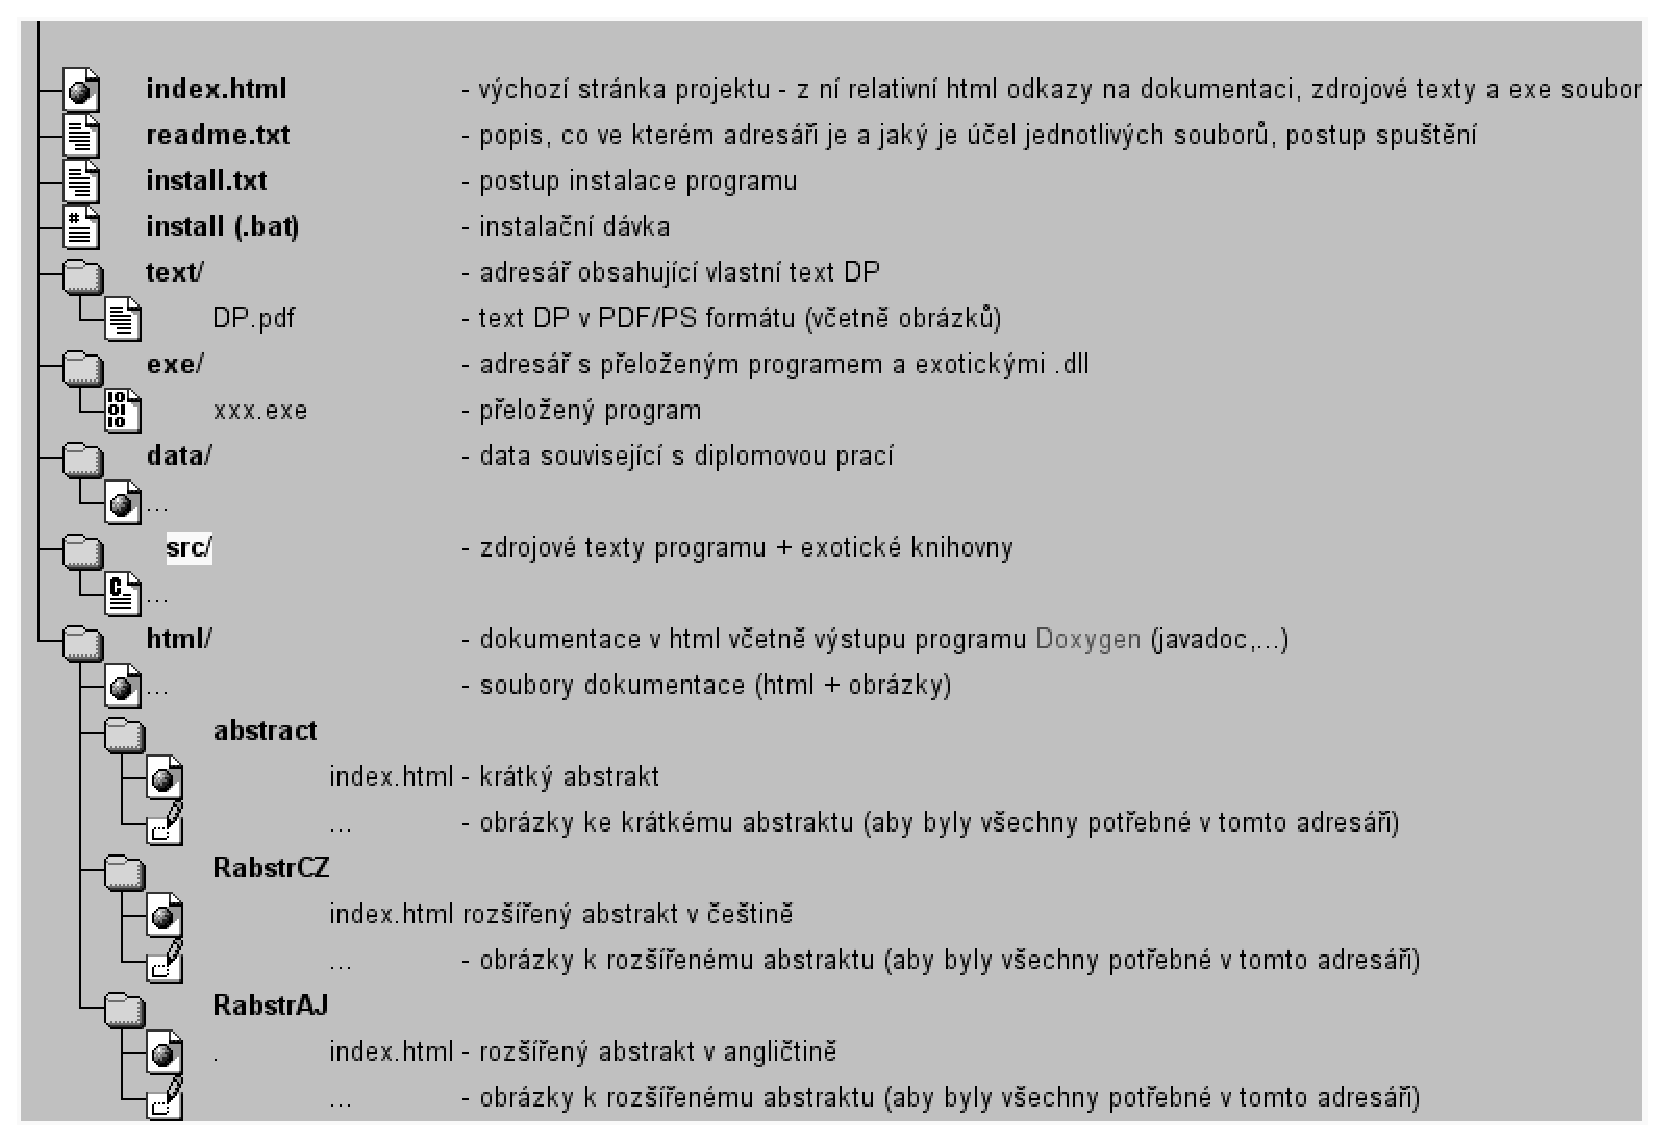
\includegraphics[width=14cm]{figures/seznamcd}
\caption{Seznam přiloženého CD --- příklad}
\label{fig:seznamcd}
\end{center}
\end{figure}

Na GNU/Linuxu si strukturu přiloženého CD můžete snadno vyrobit příkazem:\\ 
\verb|$ tree . >tree.txt|\\
Ve vzniklém souboru pak stačí pouze doplnit komentáře.

Z~\textbf{README.TXT} (případne index.html apod.)  musí být rovněž zřejmé, jak programy instalovat, spouštět a~jaké
požadavky mají tyto programy na hardware.

Adresář \textbf{text}  musí obsahovat soubor s~vlastním textem práce v~PDF nebo PS formátu, který bude později použit
pro prezentaci diplomové práce na WWW.

\end{document}
